\chapter{基于Sigma协议的身份识别与签名}

在上一章中,我们研究了身份识别协议。特别是在 \ref{subsubsec:18-6-1-1} 小节中,我们展示了如何使用安全的签名方案来建立一个挑战-应答身份识别方案,该方案提供了最高级别的安全,即针对主动攻击的安全(见定义18.8)。在本章中,我们考虑相反的方向。

首先,我们使用一种完全不同的技术开发了一种新的身份识别协议,它实现了对窃听攻击的安全性(见定义18.6)。这个协议本身就很有意义,因为它相当优雅,而且可以在DL假设下被证明是安全的。

其次,我们展示了如何将该协议转化为一个非常有效的签名方案,即\textbf{Schnorr签名方案}。在DL假设下,该方案在随机预言机模型下是安全的。

第三,我们归纳这些技术并引入了\textbf{Sigma协议}的概念。我们利用这些更普适的技术开发了几个新的身份识别协议和签名方案。

在下一章中,我们将这些技术用于更高级的用途,设计出允许一方向另一方证明某些事实是真实的协议,同时不透露任何不必要的信息。例如,我们将展示如何证明加密值$m$位于某个范围内而不透露关于$m$的任何其他信息。

\section{Schnorr身份识别协议}

我们首先描述一种称为\textbf{Schnorr身份识别}的安全的身份识别协议。如果假定离散对数问题是困难的,那么该协议对窃听攻击是安全的。

令 $\mathbb{G}$ 是一个 $q$ 阶循环群,其中 $q$ 是素数,$g\in\mathbb{G}$ 是一个生成元。假设证明者 $P$ 有一个私钥 $\alpha\in\mathbb{Z}_q$,且与之对应的公钥为 $u=g^{\alpha}\in\mathbb{G}$。为了向验证者 $V$ 证明自己的身份,$P$ 想让 $V$ 相信自己知道 $\alpha$。最简单的方法是 $P$ 直接将 $\alpha$ 发送给 $V$。这个方法其实就是我们在\ref{sec:18-3} 中讨论过的口令协议版本 1,此时函数 $H(\alpha):=g^\alpha$扮演单向函数的角色。尽管这个协议提供了针对直接攻击的安全性,但它对窃听攻击是完全不安全的。相对, Schnorr 协议是一个经过巧妙设计的交互式协议,它允许 $P$ 说服 $V$ 相信自己知道以 $g$ 为基数的离散对数 $u$,但又并不需要真的将这个值发送给 $V$。

下面是它的工作原理。令 $\mathcal{C}\subset\mathbb{Z}_q$,则Schnorr身份识别协议 $\mathcal{I}_{\rm sch}=(G,P,V)$ 的原理如下:
\begin{itemize}
	\item 密钥生成算法 $G$ 按如下方式运行:
		$$\alpha\overset{\rm R}\leftarrow\mathbb{Z}_q, ~~ u\leftarrow g^\alpha$$
		验证密钥为 $vk:=u$,私钥为 $sk:=\alpha$。
	\item $P$ 与 $V$ 之间的协议按照下面的方式运行。其中证明者 $P$ 由 $sk=\alpha$ 初始化,验证者 $V$ 由 $vk=u$ 初始化:
	\begin{enumerate}
		\item $P$ 计算 $\alpha_{\rm t}\overset{\rm R}\leftarrow\mathbb{Z}_q$,$u_{\rm t}\leftarrow g^{\alpha_{\rm t}}$,并将 $u_{\rm t}$ 发送给 $V$;
		\item $V$ 计算 $c\overset{\rm R}\leftarrow\mathcal{C}$,并将 $c$ 发送给 $P$;
		\item $P$ 计算 $\alpha_{\rm z}\leftarrow \alpha_{\rm t}+\alpha c\in \mathbb{Z}_q$,并将 $\alpha_{\rm z}$ 发送给 $V$;
		\item $V$ 检查 $g^{\alpha_{\rm z}}=u_{\rm t}\cdot u^c$ 是否成立,如果成立就输出 $\mathsf{accept}$,否则输出 $\mathsf{reject}$。
	\end{enumerate}
\end{itemize}
图 \ref{fig:19-1} 展示了该协议的工作流程。

\begin{figure}
  \centering
  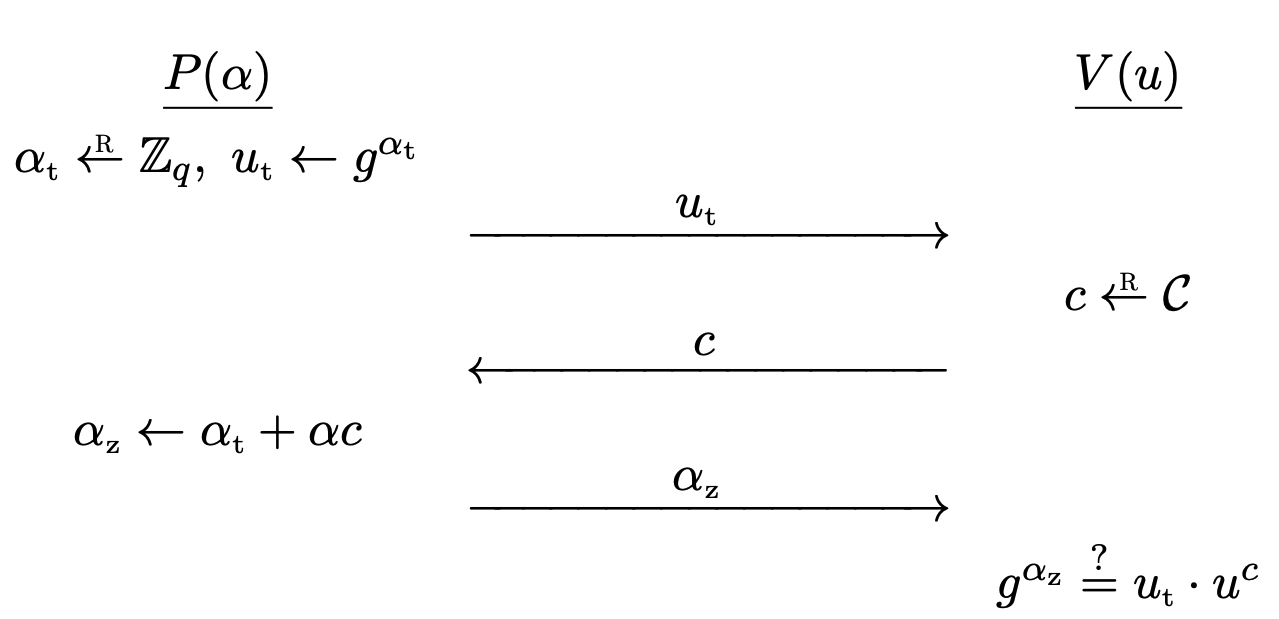
\includegraphics[width=0.55\linewidth]{figures/chapter19/fig1.png}
  \caption{Schnorr身份识别协议}
  \label{fig:19-1}
\end{figure}

$P(\alpha)$ 和 $V(u)$ 之间的一次交互产生一个\textbf{对话 (conversation)} $(u_{\rm t},c,\alpha_{\rm z})\in \mathbb{G}\times \mathcal{C}\times \mathbb{Z}_q$。如果 $V$ 的检查通过,即$g^{\alpha_{\rm z}}=u_{\rm t}\cdot u^c$ 成立,我们就称该对话为 \textbf{$u$ 的接受对话 (accepting conversation for $u$)}。不难看出,$P$ 和 $V$ 之间的交互总是能够产生一个接受对话,因为如果有 $u_{\rm t}=g^{\alpha_{\rm t}}$ 且 $\alpha_{\rm z}=\alpha_{\rm t}+\alpha c$,则有:
$$g^{\alpha_{\rm z}}=g^{\alpha_{\rm t}+\alpha c}=g^{\alpha_{\rm t}}\cdot (g^\alpha)^c=u_{\rm t}\cdot u^c$$
因此,Schnorr 协议能够满足身份识别协议所必需的基本正确性要求。

我们称集合 $\mathcal{C}$ 为\textbf{挑战空间 (challenge space)}。为了满足安全需求,我们要求 $|\mathcal{C}|$ 是超多项式的。事实上我们可以简单地取 $\mathcal{C}$ 为 $\mathbb{Z}_q$,但是技术上也可以允许更小的挑战空间。尽管我们最终会证明Schnorr协议在DL假设下对窃听攻击是安全的,但我们现在先从一个更简单的定理开始,它只证明了Schnorr协议对\emph{直接}攻击的安全性(攻击游戏 \ref{game:18-1})。

在证明这一点时,我们将表明,任何能够以不可忽略的概率成功执行直接仿冒攻击的对手,都能被转换成一个从验证密钥 $u$ 中高效地恢复私钥 $\alpha$的算法。由于这个原因,Schnorr的协议有时也被称为离散对数的知识证明。

\begin{theorem}\label{theo:19-1}
	基于 $\mathbb{G}$ 上的离散对数假设,假设 $N:=|\mathcal{C}|$ 是超多项式的,Schnorr 身份认证协议对直接攻击是安全的。
	\begin{quote}
		特别地,假设 $\mathcal{A}$ 是一个有效冒充对手,它通过攻击游戏 \ref{game:18-1} 中的直接攻击方式攻击 $\mathcal{I}_{\rm sch}$ 的优势为 $\epsilon:={\rm ID1\mathsf{adv}}[\mathcal{A},\mathcal{I}_{\rm sch}]$。那么必然存在一个有效的离散对数对手 $\mathcal{B}$,其运行时间大致是 $\mathcal{A}$ 的两倍,其优势为 $\epsilon':={\rm DL\mathsf{adv}}[\mathcal{B},\mathbb{G}]$,并且有:
	\end{quote}
	\begin{equation}\label{eq:19-1}
		\epsilon'\geq \epsilon^2-\frac{\epsilon}{N}
	\end{equation}
	\begin{quote}
		也即:
	\end{quote}
	\begin{equation}\label{eq:19-2}
		\epsilon\leq\frac{1}{N}+\sqrt{\epsilon'}
	\end{equation}
\end{theorem}

\begin{proof}[证明思路]
假设攻击游戏 \ref{game:18-1} 中的对手 $\mathcal{A}$ 在攻击 $\mathcal{I}_{\rm sch}$ 时有优势 $\epsilon$。在该游戏中,挑战者生成验证密钥 $u=g^\alpha$。在对手 $\mathcal{A}$ 的冒充尝试中,它基于某个任意的对手策略生成了协议的第一条交互信息 $u_{\rm t}$。为了赢得游戏,对手 $\mathcal{A}$ 必须用一个有效应答 $\alpha_{\rm z}$ 来响应随机挑战 $c\in\mathcal{C}$,使得 $g^{\alpha_{\rm z}}=u_{\rm t}\cdot u^c$。直观地讲,如果 $\mathcal{A}$ 能以概率 $\epsilon$ 对一个这样的随机挑战产生一个有效应答,那么它就应该能以概率 $\epsilon^2$ 对\emph{两个}随机挑战产生一个有效的应答。要使这一直觉变得严谨,需要一个有点技术性的论证,我们将在随后的引理中给出。

下面,我们先介绍如何使用 $\mathcal{A}$ 计算随机数 $u\in\mathbb{G}$ 的离散对数。我们使用 $u$ 作为 $\mathcal{I}_{\rm sch}$ 的验证密钥,并让 $\mathcal{A}$ 生成协议的第一条交互 $u_{\rm t}$。然后我们向 $\mathcal{A}$ 提供一个随机挑战 $c$,并希望 $\mathcal{A}$ 产生一个有效应答 $\alpha_{\rm z}$。如果这确实发生了,我们就将 $\mathcal{A}$ 的内部状态``回溯"到它刚刚生成 $u_{\rm t}$ 后的那一刻,然后给 $\mathcal{A}$ 提供另一个随机挑战 $c'$,并希望 $\mathcal{A}$ 产生另一个有效应答 $\alpha_{\rm z}'$。

如果上面这些都发生了,那么对于一个给定的验证密钥 $u$,我们就得到了两个接受对话 $(u_{\rm t},c,\alpha_{\rm z})$ 和 $(u_{\rm t},c',\alpha_{\rm z}')$,且这两个对话的第一条交互 $u_{\rm t}$ 相同。此外,由于 $\mathcal{C}$ 是超多项式的,因此我们可以以压倒性的概率得到 $c'\neq c$ 。基于以上信息,我们可以很容易地计算出 ${\rm \mathsf{Dlog}}_gu$。事实上,由于上面的两个对话都是接受对话,我们有下面两个等式:
$$g^{\alpha_{\rm z}}=u_{\rm t}\cdot u^c,~~~~
g^{\alpha_{\rm z}'} =u_{\rm t}\cdot u^{c'}$$
用第一式除以第二式, $u_{\rm t}$ 就被抵消了,于是我们有:
\begin{equation}\label{eq:19-3}
	g^{\Delta\alpha}=u^{\Delta c}
\end{equation}
其中$\Delta\alpha:=\alpha_{\rm z}-\alpha_{\rm z}'$,$\Delta c:=c-c'$。由于 $\Delta c\neq 0$,且循环群 $\mathbb{G}$ 的阶 $q$ 是素数,所以倒数 ${1}/{\Delta c}$ 存在于 $\mathbb{Z}_q$ 中。我们可以将式 \ref{eq:19-3} 中等式的左右两边都升阶 ${1}/{\Delta c}$,于是有:
	$$g^{{\Delta\alpha}/{\Delta c}}=u$$
因此,我们可以有效计算离散对数 ${\rm \mathsf{Dlog}}_gu$,其值为 ${\Delta\alpha}/{\Delta c}$。

读者应该注意到,这里提出的从两个接受对话中提取离散对数的技术,与事实 10.3 中使用的想法基本相同。事实上,使用 10.6.1 节中的术语,我们可以看到 $(\alpha_{\rm z},-c)$ 和 $(\alpha_{\rm z}',-c')$ 是 $u_{\rm t}$ 相对于$g$ 和 $u$ 的不同表示。事实 10.3 告诉了我们如何从这两个表示中计算出 ${\rm \mathsf{Dlog}}_gu$。
\end{proof}

这个定理与我们在本文中迄今为止所介绍的所有其他安全定理有着质的不同。事实上,在这个定理的证明中,虽然我们表明每个攻击 $\mathcal{I}_{\rm sch}$ 的对手 $\mathcal{A}$ 都可以转化为破解离散对数问题的对手 $\mathcal{B}$,但我们构造的对手 $\mathcal{B}$ \emph{并不是} $\mathcal{A}$ 的基本包装器,因为对手 $\mathcal{B}$ 要运行 $\mathcal{A}$ \emph{两次}。此外,这个定理在量上也是不同的,因为安全归约根本就不是很严密:如果 $\mathcal{A}$ 以概率 $\epsilon$ 获胜,那么 $\mathcal{B}$ 只能保证以 $\approx\epsilon^2$ 的概率获胜。

因此,为了使上述想法更严谨,我们需要先引入下面的引理:

\begin{lemma}[回溯引理]\label{theo:19-2}
	令 $S$ 和 $T$ 是两个非空有限集,$f:S\times T\to\{0,1\}$ 是一个函数。令 $\mathsf{X}$、$\mathsf{Y}$ 和 $\mathsf{Y}'$ 是相互独立的随机变量,其中 $\mathsf{X}$ 在集合 $S$ 中取值,$\mathsf{Y}$ 和 $\mathsf{Y}'$ 都在 $T$ 上均匀分布。令 $\epsilon:=\Pr[f(\mathsf{X},\mathsf{Y})=1]$,$N:=|T|$,则有:
	$$\Pr[f(\mathsf{X},\mathsf{Y})=1\land f(\mathsf{X},\mathsf{Y}')=1\land \mathsf{Y}\neq\mathsf{Y}']\geq\epsilon^2-\frac{\epsilon}{N}$$
\end{lemma}

\begin{proof}
	对于每个 $s\in S$,令 $g(s):=\Pr[f(s,\mathsf{Y})=1]$。首先,我们可以观察到 $E[g(\mathsf{X})]=\epsilon$,这是因为:
	\begin{equation*}
		\begin{aligned}
			E[g(\mathsf{X})]
			&=\sum_{s\in S}g(s)\Pr[\mathsf{X}=s]=\sum_{s\in S}\Pr[f(s,\mathsf{Y})=1]\Pr[\mathsf{X}=s]\\
			&=\sum_{s\in S}\Pr[f(s,\mathsf{Y})=1\land \mathsf{X}=s] \text{ \emph{(独立性)}}\\
			&=\sum_{s\in S}\Pr[f(\mathsf{X},\mathsf{Y})=1\land \mathsf{X}=s]\\
			&=\Pr[f(\mathsf{X},\mathsf{Y})=1] \text{ \emph{(全概率)}}\\
			&=\epsilon
		\end{aligned}
	\end{equation*}
	
	其次,考虑一个固定的 $s∈S$,令 $\mathcal{U}_s$ 为 $f(s,\mathsf{Y})=1\land f(s,\mathsf{Y}')=1\land \mathsf{Y}\neq\mathsf{Y}'$ 成立的事件,我们称:
	$$
	\Pr[\mathcal{U}_s]=g(s)^2-\frac{g(s)}{N}
	$$
	为了证明这一点,令 $N_s$ 是满足 $f(s, t)=1$ 的 $t\in T$ 的数量,那么有 $N_s$ 种方法可以选择满足 $f(s,\mathsf{Y})=1$ 的 $\mathsf{Y}$。而对于每个 $\mathsf{Y}$ 的选择,有 $N_s-1$ 种方法可以选择满足 $f(s,\mathsf{Y}')=1\land \mathsf{Y}\neq\mathsf{Y}'$ 的 $\mathsf{Y}'$。由于 $g(s)={N_s}/{N}$,因此我们有:
	$$
	\Pr[\mathcal{U}_s]=\frac{N_s(N_s-1)}{N^2}=\frac{N_s^2}{N^2}-\frac{N_s}{N^2}=g(s)^2-\frac{g(s)}{N}
	$$

	最后,令 $\mathcal{U}$ 为 $f(\mathsf{X},\mathsf{Y})=1\land f(\mathsf{X},\mathsf{Y}')=1\land \mathsf{Y}\neq\mathsf{Y}'$ 成立的事件,我们有:
	\begin{equation*}
		\begin{aligned}
			\Pr[\mathcal{U}]
			&=\sum_{s\in S}\Pr[\mathcal{U}\land\mathsf{X}=s]\text{ \emph{(全概率)}}\\
			&=\sum_{s\in S}\Pr[f(s,\mathsf{Y})=1\land f(s,\mathsf{Y}')=1\land \mathsf{Y}\neq\mathsf{Y}'\land\mathsf{X}=s]\\
			&=\sum_{s\in S}\Pr[f(s,\mathsf{Y})=1\land f(s,\mathsf{Y}')=1\land \mathsf{Y}\neq\mathsf{Y}']\cdot\Pr[\mathsf{X}=s]\text{ \emph{(独立性)}}\\
			&=\sum_{s\in S}\Pr[\mathcal{U}_s]\cdot\Pr[\mathsf{X}=s]=\sum_{s\in S}[g(s)^2-\frac{g(s)}{N}]\cdot\Pr[\mathsf{X}=s]\\
			&=E[g(\mathsf{X})^2]-\frac{g(\mathsf{X})}{N}\\
			&\geq E[g(\mathsf{X})]^2-\frac{E[g(s)]}{N}=\epsilon^2-\frac{\epsilon}{N}
		\end{aligned}
	\end{equation*}
	上面我们使用了这样一个一般事实:对于任意随机变量 $\mathsf{Z}$ 都有 $E[\mathsf{Z}^2]\geq E[\mathsf{Z}]^2$,在这里我们的这个 $\mathsf{Z}=g(\mathsf{X})$。这是詹森不等式的一个特例。
\end{proof}

\begin{proof}[定理 \ref{theo:19-1} 的证明]
	利用具有优势 $\epsilon$ 的冒充对手 $\mathcal{A}$ ,我们能够建立一个具有优势 $\epsilon'$ 的 DL 对手 $\mathcal{B}$,如下所示。对手 $\mathcal{B}$ 从其挑战者那里得到一个 DL 问题实例 $u = g^\alpha$,而我们的目标是让 $\mathcal{B}$ 在 $\mathcal{A}$ 的帮助下计算出 $\alpha$。$\mathcal{B}$ 的计算过程可以分为两个阶段。

在第一阶段,$\mathcal{B}$ 扮演 $\mathcal{A}$ 的挑战者的角色,将 $u$ 的值交给 $\mathcal{A}$ 作为验证公钥。在这一步中,$\mathcal{B}$ 的目标是计算出两个具有不同挑战的 $u$ 的接受对话,即:
$$(u_{\rm t},c,\alpha_{\rm z}),~~(u_{\rm t},c',\alpha_{\rm z}')$$
其中:
$$g^{\alpha_{\rm z}}=u_{\rm t}\cdot u^c,~~
g^{\alpha_{\rm z}'}=u_{\rm t}\cdot u^{c'},~~
c\neq c'$$

以下是 $\mathcal{B}$ 做到这一点的方法:
\begin{enumerate}
	\item $\mathcal{A}$ 扮演证明者,并将 $u_{\rm t}$ 发送给扮演验证者的 $\mathcal{B}$;
	\item $\mathcal{B}$ 向 $\mathcal{A}$ 发送一个随机数 $c\in\mathcal{C}$;
	\item $\mathcal{A}$ 向 $\mathcal{B}$ 发送 $\alpha_{\rm z}$;
	\item $\mathcal{B}$ 对 $\mathcal{A}$ 进行``回溯"操作,使 $\mathcal{A}$ 的内部状态与步骤 1 结束时完全相同,然后 $\mathcal{B}$ 向 $\mathcal{A}$ 发送一个新的随机数 $c'\in\mathcal{C}$;
	\item $\mathcal{A}$ 向 $\mathcal{B}$ 发送 $\alpha_{\rm z}'$。
\end{enumerate}
下面我们应用回溯引理 \ref{theo:19-2}。在该引理中,随机变量 $\mathsf{Y}$ 与挑战 $c$ 对应,$\mathsf{Y}'$ 与挑战 $c'$ 对应,$\mathsf{X}$ 与 $\mathcal{A}$ 、$\mathcal{B}$ 和 $\mathcal{B}$ 的挑战者的所有其他随机选择对应,具体包括群 $\mathbb{G}$ 和群元素 $g,u,u_t\in\mathbb{G}$。当产生的对话是 $u$ 的一个接受对话时,引理中的函数 $f$ 为 $1$,否则就为 $0$。因此,如果 $(u_{\rm t},c,\alpha_{\rm z})$ 是 $u$ 的接受对话,则 $f(\mathsf{X},\mathsf{Y})=1$,如果 $(u_{\rm t},c',\alpha_{\rm z}')$ 是 $u$ 的接受性对话,则 $f(\mathsf{X},\mathsf{Y}')=1$。应用该引理,我们发现 $\mathcal{B}$ 得到两个不同挑战的接受对话的概率至少为 $\epsilon^2-{\epsilon}/{N}$。

所以现在假设 $\mathcal{B}$ 已经成功计算出两个这样的接受对话 $(u_{\rm t},c,\alpha_{\rm z})$ 和 $(u_{\rm t},c',\alpha_{\rm z}')$。在第二阶段,$\mathcal{B}$ 用这两个对话来计算 $\alpha$。事实上,正如在上面的证明思路中已经讨论过的,我们可以计算$\alpha={\Delta\alpha}/{\Delta c}$,其中$\Delta\alpha:=\alpha_z-\alpha_z'$,$\Delta c:=c-c'$。

这就得到了式 \ref{eq:19-1}。下面我们论证式 \ref{eq:19-2} 可由式 \ref{eq:19-1} 推出。为此,我们不妨假设 $\epsilon\geq{1}/{N}$,否则式 \ref{eq:19-2} 显然是成立的。因此我们有:
$$
\begin{aligned}
	(\epsilon-\frac{1}{N})^2
	&=\epsilon^2-\frac{2\epsilon}{N}+\frac{1}{N^2}\leq\epsilon^2-\frac{2\epsilon}{N}+\frac{\epsilon}{N} \text{\emph{ (因为 }}\epsilon\geq\frac{1}{N}\text{\,)}\\
	&=\epsilon^2-\frac{\epsilon}{N}\leq \epsilon' \text{ \emph{(式}\ref{eq:19-1} \emph{)}}
\end{aligned}
$$
因此式 \ref{eq:19-2} 得证。

回顾一下,我们展示了如何从恶意验证者 $\mathcal{A}$ 中有效地\emph{提取}私钥 $\alpha$,进而证明了针对直接攻击的安全性。这使我们能够利用恶意验证者来解决$\mathbb{G}$中的离散对数问题。我们的\emph{提取器}通过回溯证明者的状态来获得两个接受对话 $(u_{\rm t},c,\alpha_{\rm z})$ 和 $(u_{\rm t},c',\alpha_{\rm z}')$,其中 $c\neq c'$。在安全性证明中回溯证明者 $\mathcal{A}$ 是可能的,因为我们完全控制了 $\mathcal{A}$ 的执行环境。在现实世界中,由于不能对诚实证明 $P$ 进行回溯,攻击者就不能使用这种策略从 $P$ 那里提取私钥。
\end{proof}

\subsection{诚实验证者零知识和针对窃听的安全性}\label{subsec:19-1-1}

我们已经证明了在离散对数假设下,Schnorr 协议对\emph{直接}攻击是安全的。事实上在相同的假设下,Schnorr 协议对于\emph{窃听}攻击也是安全的。现在,在某次窃听攻击中,对手获得了 $vk$ 和一张记录列表,该表的内容是$P$(在输入$sk$上)与 $V$(在输入$vk$上)之间的若干对话。我们的想法是证明这些对话对于对手来说没有任何帮助,因为在给定 $vk$ 而没有给定 $sk$ 的情况下,对手也可以自己有效地生成这些对话。如果我们能证明这一点,我们也就大功告成了。事实上,假设 $\mathcal{A}$ 是一个对手,它通过窃听成功发动仿冒攻击的优势是不可忽略不计的。然后,我们用另一个对手 $\mathcal{B}$ 来替代 $\mathcal{A}$,它的工作方式与 $\mathcal{A}$ 是一样的,只是现在 $\mathcal{B}$ 自己生成了对话列表,而不是从挑战者那里获取记录。这样,$\mathcal{B}$ 就发动了一个直接攻击,但是它与发动仿冒攻击的 $\mathcal{A}$ 具有相同的优势。

下面,我们将上面的想法扩展到更一般的情况,引入\textbf{诚实验证者零知识} 的概念。

\begin{definition}
	令 $\mathcal{I}=(G,P,V)$ 是一个身份识别协议。如果存在一个有效的概率性算法 $Sim$(称为\textbf{模拟器 simulator})使得对于 $G$ 的任意可能输出 $(vk,sk)$,$Sim$ 在输入 $vk$ 上的输出分布与 $P$ (在输入$sk$上)与 $V$(在输入$vk$上) 之间对话记录的分布相同,我们就称 $\mathcal{I}$ 是\textbf{诚实验证者零知识 (honest verifier zero knowledge, HVZK)} 的。
\end{definition}

下面,我们对其中的一些术语进行说明。所谓``零知识"的意思是,对手从 $P$ 那里什么也学不到,因为对手可以在不知道 $sk$ 的情况下自己使用算法 $Sim$ 模拟对话。而``诚实验证者"表达了这样一个事实,即这种模拟只对 $P$ 和\emph{诚实的}验证者 $V$ 之间的对话有效,而对于\emph{非诚实}的验证者,比如\emph{主动}攻击中可能出现的验证者,都是无效的。零知识的概念,包括诚实验证者零知识以及许多其他的变体,还会出现在身份识别协议之外的许多其他类型的协议中。

\begin{theorem}\label{theo:19-3}
	如果一个身份识别协议 $\mathcal{I}=(G,P,V)$ 对于直接攻击是安全的,且该协议是 HVZK 的,那么该协议对于窃听攻击也是安全的。
	\begin{quote}
		特别地,如果 $\mathcal{I}$ 是带有模拟器 ${Sim}$ 的 HVZK,那么对于每一个通过攻击游戏 18.2 中的窃听攻击来攻击 $\mathcal{I}$ 的冒充对手 $\mathcal{A}$,如果 $\mathcal{A}$ 最多能获得 $Q$ 次交互记录,必然存在一个通过攻击游戏 \ref{game:18-1} 中的直接攻击来攻击 $\mathcal{I}$ 的对手 $\mathcal{B}$,其中 $\mathcal{B}$ 是 $\mathcal{A}$ 的一个基本包装器,并且 $\mathcal{B}$ 最多运行 $Q$ 次 ${Sim}$,使得:
		$${\rm ID2\mathsf{adv}}[\mathcal{A},\mathcal{I}]=
			{\rm ID1\mathsf{adv}}[\mathcal{B},\mathcal{I}]$$
	\end{quote}
\end{theorem}

\begin{proof}
	$\mathcal{B}$ 的工作方式与 $\mathcal{A}$ 相同,只是它不是从挑战者那里获得交互记录,而是用 ${Sim}$ 自己生成交互记录。对手 $\mathcal{B}$ 的工作方式如图 \ref{fig:19-2} 所示。
\end{proof}

\begin{figure}
  \centering
  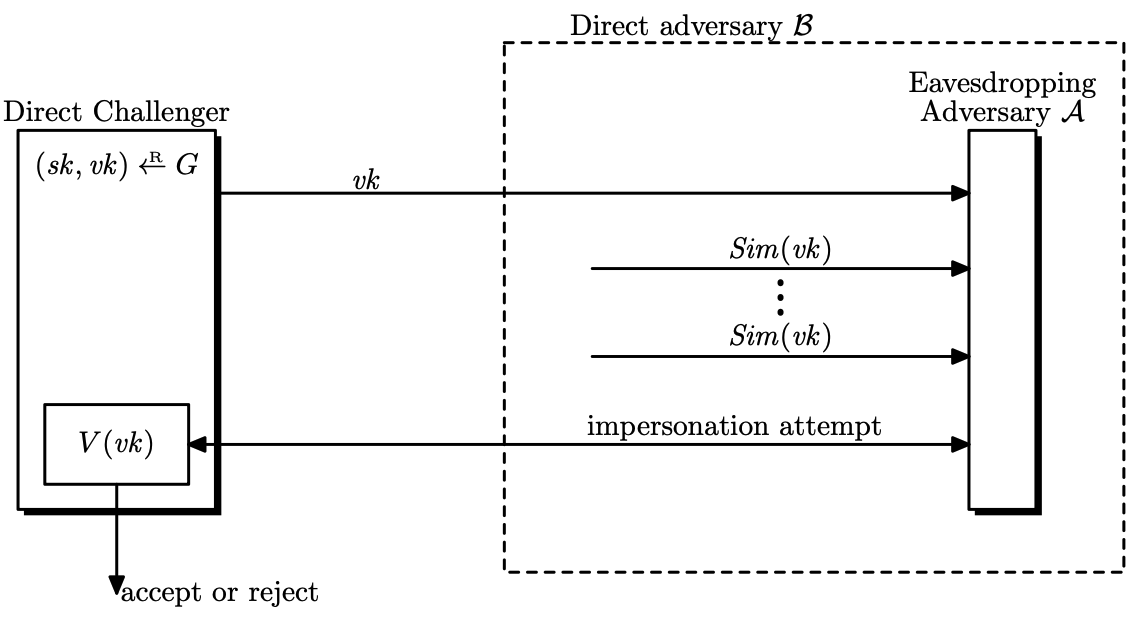
\includegraphics[width=0.65\linewidth]{figures/chapter19/fig2.png}
  \caption{定理 \ref{theo:19-3} 的证明中的对手 $\mathcal{B}$}
  \label{fig:19-2}
\end{figure}

下面让我们回到 Schnorr 身份识别协议。

\begin{theorem}\label{theo:19-4}
	Schnorr 身份识别协议是 HVZK 的。
\end{theorem}

\begin{proof}
	证明的思路是在生成模拟对话 $(u_{\rm t},c,\alpha_{\rm z})$ 时,我们不需要像 $P$ 和 $V$ 之间的真实对话那样,按照给定的顺序生成对话中的消息。事实上,模拟器 ${Sim}$ 是以\emph{倒序}生成信息的。在输入 $vk=u$ 时,模拟器 ${Sim}$ 计算:
		$$\alpha_{\rm z}\overset{\rm R}\leftarrow\mathbb{Z}_q,~~
		c\overset{\rm R}\leftarrow\mathcal{C},~~
		u_{\rm t}\leftarrow\frac{g^{\alpha_{\rm z}}}{u^c}$$
	并输出对话 $(u_{\rm t},c,\alpha_{\rm z})$。
	
	现在我们论证 ${Sim}$ 在输入 $vk=u$ 上的输出具有正确的分布。一个关键性的观察是,在真实交互中,$c$ 和 $\alpha_{\rm z}$ 是相互独立的,$c$ 在 $\mathcal{C}$ 上均匀分布,而 $\alpha_z$ 在 $\mathbb{Z}_q$ 上均匀分布。此外,给定 $c$ 和 $\alpha_{\rm z}$,$u_{\rm t}$ 的值可由等式 $g^{\alpha_{\rm z}}=u_{\rm t}\cdot u^c$ 唯一确定。而这显然与模拟器的输出分布相同。
\end{proof}

作为一个推论,我们立即可以得到:

\begin{theorem}\label{theo:19-5}
	如果 Schnorr 身份识别协议对直接攻击是安全的,那么它对窃听攻击也是安全的。
	
	\begin{quote}
		特别地,对于每个通过攻击游戏 18.2 中的窃听攻击来攻击 $\mathcal{I}_{\rm sch}$ 的冒充对手 $\mathcal{A}$,都有一个通过攻击游戏 \ref{game:18-1} 中的直接攻击来攻击 $\mathcal{I}_{\rm sch}$ 的对手 $\mathcal{B}$,其中 $\mathcal{B}$ 是 $\mathcal{A}$ 的一个基本包装器,满足:
		$${\rm ID2\mathsf{adv}}[\mathcal{A},\mathcal{I}_{\rm sch}]=
		{\rm ID1\mathsf{adv}}[\mathcal{B},\mathcal{I}_{\rm sch}]$$
	\end{quote}
\end{theorem}

乍看之下,我们关于 Schnorr 协议的结论似乎是反直觉的,甚至可能是矛盾的。在只知道 $vk$ 的情况下,怎么可能既很难进行冒充攻击,又容易产生对话呢?答案是,在进行冒充攻击时,验证者 $V$ 主动地参与对话,而消息的时间和顺序至关重要:扮演证明者的对手必须在看到 $V$ 生成的挑战 $c$ \emph{之前}生成第一条消息 $u_{\rm t}$。然而,模拟器可以自由地以任何方便的顺序生成信息:在定理 \ref{theo:19-4} 的证明中,模拟器先生成了 $c$ 和 $\alpha_{\rm z}$,然后才计算 $u_{\rm t}$。这些结果表明,如果挑战空间很小,Schnorr 协议将是完全\emph{不安全}的:在冒充尝试中,对手可以使用模拟器准备一个接受对话 $(u_{\rm t},c,\alpha_{\rm z})$,然后将 $u_{\rm t}$ 发送给 $V$,然后希望 $V$ 选择的挑战等于其准备的挑战 $c$。如果真的是这样,对手就可以用 $\alpha_{\rm z}$ 应答从而使 $V$ 接受对话。因此,以 ${1}/{|\mathcal{C}|}$ 的优势破解 Schnorr 识别协议是很容易的。所以为了确保安全性,挑战空间的大小 $|\mathcal{C}|$ 必须是超多项式的。

Schnorr 识别协议对攻击游戏 18.3 中的\emph{主动}攻击是否安全是一个开放的问题:目前还没有已知的有效主动攻击,但也没有证据可以排除离散对数假设下的这种攻击。在本章的稍后部分,我们将介绍一个对Schnorr身份识别的细小变化,它被证明在DL假设下对主动攻击是安全的。
\section{从身份识别协议到签名}\label{sec:19-2}

在本节中,我们将展示如何将 Schnorr 协议转换为一个签名方案。在离散对数假设下,该签名方案在随机预言机模型下是安全的。在本章的稍后部分,我们将看到这个构造实际上是一个更一般的结构的一个具体实例。

我们从 Schnorr 识别协议 $\mathcal{I}_{\rm sch}$ 开始,它定义在阶为素数 $q$ 的循环群 $\mathbb{G}$ 上,该群有生成元 $g\in\mathbb{G}$。此外,其挑战空间 $\mathcal{C}\subseteq\mathbb{Z}_q$。除此之外,我们还需要一个哈希函数 $H:\mathcal{M}\times\mathbb{G}\to\mathcal{C}$,该函数在安全证明中被建模为一个随机预言机。这里的 $\mathcal{M}$ 将会是签名方案的消息空间。

签名方案的构造思想是,对于消息 $m\in\mathcal{M}$ 的签名是一个元组 $(u_{\rm t},\alpha_{\rm z})$,其中 $(u_{\rm t},c,\alpha_{\rm z})$ 是在 Schnorr 识别协议 $\mathcal{I}_{\rm sch}$ 中对验证密钥 $u$ 的接受对话,挑战则来自 $c\leftarrow H(m,u_{\rm t})$。直观地讲,哈希函数 $H$ 在这里扮演 Schnorr 身份识别协议中验证者的角色。

具体地,Schnorr 签名方案为 $\mathcal{S}_{\rm sch}=(G,S,V)$,其中:
\begin{itemize}
	\item 密钥生成算法 $G$ 按如下方式运行:
	    \[
	    \alpha\overset{\rm R}\leftarrow\mathbb{Z}_q,
	    \quad
	    u\leftarrow g^\alpha
	    \]
	    其中公钥为 $pk:=u$,私钥为 $sk:=\alpha$。
	\item 为了使用私钥 $sk=\alpha$ 对消息 $m\in\mathcal{M}$ 进行签名,签名算法 $S$ 按如下方式运行:
		\[
		\alpha_{\rm t}\overset{\rm R}\leftarrow\mathbb{Z}_q,
		\quad	
		u_{\rm t}\leftarrow g^{\alpha_{\rm t}},
		\quad
		c\leftarrow H(m,u_{\rm t}),
		\quad
		\alpha_{\rm z}\leftarrow\alpha_{\rm t}+\alpha c
		\]
		输出签名 $\sigma:=(u_{\rm t},\alpha_{\rm z})$。
	\item 为了使用公钥 $pk=u$ 验证消息 $m\in\mathcal{M}$ 的签名 $\sigma=(u_{\rm t},\alpha_{\rm z})$,签名验证算法 $V$ 计算 $c\leftarrow H(m,u_{\rm t})$,当 $g^{\alpha_{\rm z}}=u_{\rm t}\cdot u^c$ 成立时输出 $\mathsf{accept}$,否则输出 $\mathsf{reject}$。
\end{itemize}

尽管我们把签名算法描述为一种随机化算法,但这并不是必须的。练习 \ref{exer:13-6} 展示了如何对签名算法进行去随机化。这种去随机化在实践中很重要,因为它可以避免不良随机性攻击,就像练习 \ref{exer:19-1} 所展示的那样。

我们下面将要说明,如果把 $H$ 建模为一个随机预言机,那么如果 Schnorr 识别协议对窃听攻击是安全的,那么 Schnorr 签名方案也一定是安全的。而我们已经在定理 \ref{theo:19-5} 中证明了前者。然而,首先考虑窃听攻击游戏的一个稍微增强的版本是有好处的。

\subsection{一个有用的抽象:重复冒充攻击}

我们考虑一种增强版本的针对识别协议的冒充攻击,在这种攻击中,我们允许对手反复进行冒充尝试,这些冒充尝试针对的是验证者的不同实例,它们同时运行,并使用相同的验证公钥。我们可以为直接攻击、窃听攻击和主动攻击定义这个概念,但我们目前先考虑窃听攻击,因为这就是我们的应用所需要的。另外,我们只考虑无状态和有验证公钥的识别协议。

下面是攻击游戏的更多细节。

\begin{game}[$r$ 次重复冒充窃听攻击]\label{game:19-1}
给定识别协议 $\mathcal{I}=(G,P,V)$,正整数 $r$ 和对手 $\mathcal{A}$,攻击游戏按以下流程运行。其密钥生成阶段和窃听阶段与攻击游戏 18.2 完全相同。

唯一不同的是冒充阶段。现在,我们允许对手 $\mathcal{A}$ 与最多 $r$ 个验证者同时互动。挑战者扮演这些验证者的角色,他们都使用在密钥生成阶段产生的相同的验证公钥。如果对手使这些验证者中的任何一个输出 $\mathsf{accept}$,我们就称它赢得了该游戏。

我们将 $\mathcal{A}$ 对于 $\mathcal{I}$ 和 $r$ 的优势记为 ${\rm rID2\mathsf{adv}}[\mathcal{A},\mathcal{I},r]$,其值等于 $\mathcal{A}$ 赢得该游戏的概率。
\end{game}

下面的引理将表明,$r$ 次重复冒充窃听攻击等价于普通的窃听攻击。也就是说,赢得攻击游戏 \ref{game:19-1} 并不会比赢得攻击游戏 18.2 更容易。

\begin{lemma}\label{theo:19-6}
令 $\mathcal{I}$ 是一个身份识别协议。对于每个 $r$ 次重复冒充窃听攻击对手 $\mathcal{A}$,都存在一个标准窃听对手 $\mathcal{B}$,其中 $\mathcal{B}$ 是一个围绕 $\mathcal{A}$ 的基本包装器,满足:

\begin{equation}
{\rm rID2\mathsf{adv}}[\mathcal{A},\mathcal{I},r]\leq r\cdot{\rm ID2\mathsf{adv}}[\mathcal{B}, \mathcal{I}]
\end{equation}

\end{lemma}

\begin{proof}[证明简述]
这是一个简单的“猜测论证”。对手 $\mathcal{B}$ 随机选择 $\omega\in\{1,\dots,r\}$,然后扮演 $\mathcal{A}$ 的挑战者。它首先从自己的挑战者那里获得验证公钥和几条对话记录,并将这些传递给 $\mathcal{A}$。在冒充阶段,对于验证者的第 $j$ 个实例,如果 $j\neq\omega$,对手 $\mathcal{B}$ 自己扮演验证者;否则,如果 $j=\omega$,对手 $\mathcal{B}$ 就作为 $\mathcal{A}$ 和攻击游戏 18.2 中它自己的挑战者之间的简单管道。显然,$\mathcal{A}$ 在与 $\mathcal{B}$ 游戏时让其中一个验证者输出 $\mathsf{accept}$ 的概率与攻击游戏 \ref{game:19-1} 中相同。此外,如果 $\mathcal{B}$ 猜到了其中一个输出 $\mathsf{accept}$ 的验证者的索引,它就赢得了攻击游戏,这发生的概率至少是 ${1}/{r}$。
\end{proof}

\subsection{Schnorr 签名的安全性分析}

我们下面将表明,只要 Schnorr 身份识别协议对窃听攻击是安全的,Schnorr 签名方案在随机预言机模型下就是安全的。

\begin{theorem}\label{theo:19-7}
如果 $H$ 是一个随机预言机,且 Schnorr 身份识别协议对窃听攻击是安全的,那么 Schnorr 签名方案也是安全的。

\begin{quote}
特别地,令 $\mathcal{A}$ 是如攻击游戏 13.1 的随机预言机模型那样攻击  $\mathcal{S}_{\rm sch}$ 的一个对手,假设 $\mathcal{A}$ 最多发起 $Q_{\rm s}$ 次签名查询和 $Q_{\rm ro}$ 次随机预言机查询。那么必然存在一个 $(Q_{\rm ro}+1)$ 次重复冒充攻击对手 $\mathcal{B}$ 能够通过攻击游戏 \ref{game:19-1} 中的窃听攻击来攻击  $\mathcal{I}_{\rm sch}$,其中 $\mathcal{B}$ 是一个围绕 $\mathcal{A}$ 的基本包装器,满足:
\end{quote}
\begin{equation}\label{eq:19-5}
{\rm SIG^{ro}\mathsf{adv}}[\mathcal{A}, \mathcal{S}_{\rm sch}]\leq{Q_{\rm s}(Q_{\rm s}+Q_{\rm ro}+1)}/{q}+{\rm rID2\mathsf{adv}}[\mathcal{B},\mathcal{I}_{\rm sch},Q_{\rm ro}+1]
\end{equation}
\end{theorem}

\begin{proof}[证明思路]
我们的目标是将伪造签名的对手 $\mathcal{A}$ 转化为在 $r$ 次重复冒充窃听攻击中破坏 Schnorr 身份识别协议安全性的对手 $\mathcal{B}$,其中 $r:=Q_{\rm ro}+1$。

第一个想法是,我们必须以某种方式在不使用私钥的情况下响应 $\mathcal{A}$ 的签名查询。想要实现这一点,可以通过利用窃听攻击中获取的对话记录来建立所需的签名,并``修正"随机预言机 $H$,使其与签名一致。只有当随机预言机在已经被查询过的位置重新被查询时,这种修复才会失败。但由于随机预言机的输入包括一个随机群元素,因此发生的概率极低。这也就是公式 \ref{eq:19-5} 中出现 ${Q_s(Q_s+Q_{\rm ro}+1)}/{q}$ 修正项的原因。

一旦摆脱了签名查询,我们认为,如果对手成功地伪造了签名,它就可以有效地被用于对  $\mathcal{I}_{\rm sch}$ 的 $r$ 次重复冒充窃听攻击。我们再次利用了 $H$ 被建模为一个随机预言机的事实。由于签名伪造必须被包含在没有被作为签名查询而提交的信息中,因此相应的随机预言机查询必须与所有签名查询的位置相异。由于伪造签名与签名查询不能同时作为同一条消息提交,因此相应的随机预言机查询必须与所有签名查询的位置相异。所以,该位置上随机预言机的输出值在身份识别协议的运行中基本上可以视作一个随机挑战。我们事先并不知道哪一个随机预言机查询对应于一个伪造签名,这就是我们必须使用 $r$ 次重复冒充窃听攻击游戏的原因。
\end{proof}

\begin{proof}
为了简化分析,我们将假设当 $\mathcal{A}$ 输出一个伪造签名 $(m,\sigma)$,$\sigma=(u_{\rm t},\alpha_{\rm z})$ 时,$\mathcal{A}$ 一定已经在 $(m,u_{\rm t})$ 这一点上显式地查询了随机预言机。如有必要,我们会修改 $\mathcal{A}$ 以确保这种情况,以使得修改后的 $\mathcal{A}$ 所进行的随机预言机查询次数最多为 $Q_{\rm ro}+1$。

我们下面将定义两个攻击游戏。游戏 0 基本上就是原始的签名攻击游戏,其中 $H$ 被建模为一个随机预言机。游戏 1 是一个少量修改后的版本。对于 $j=0,1$,我们记 $W_j$ 是 $\mathcal{A}$ 在游戏 $j$ 中获胜的事件。

\noindent
\textbf{游戏 0。}
挑战者的工作方式与攻击游戏 13.1 的随机预言机版本相同。与往常一样,我们用一个关联数组 $Map:\mathcal{M}\times\mathbb{G}\to\mathcal{C}$ 来实现随机预言机。我们还维护一个关联数组 $Explicit:\mathcal{M}\times\mathbb{G}\to\mathbb{Z}$ 以记录那些随机预言机第一次被对手显式查询的位置,而不包含被签名算法隐式地查询的位置。挑战者的工作逻辑如图 \ref{fig:19-3}。

\begin{figure}
  \hspace*{45pt} 初始化:\\
  \hspace*{70pt} 令 $\alpha\overset{\rm R}\leftarrow\mathbb{Z}_q$,计算 $u\leftarrow g^\alpha$\\
  \hspace*{70pt} 初始化两个空的关联数组 $Map:\mathcal{M}\times\mathbb{G}\to\mathcal{C}$ 和 $Explicit:\mathcal{M}\times\mathbb{G}\to\mathbb{Z}$\\
  \hspace*{70pt} 将公钥 $u$ 发送给 $\mathcal{A}$;\\
  \hspace*{45pt} 当收到第 $i$ 个签名查询 $m_i\in\mathcal{M}$ 时:\\
  \hspace*{70pt} 令 $\alpha_{{\rm t}i}\overset{\rm R}\leftarrow\mathbb{Z}_q$,$c_i\overset{\rm R}\leftarrow\mathcal{C}$,计算 $u_{{\rm t}i}\leftarrow g^{\alpha_{{\rm t}i}}$\\
  \hspace*{30pt} (1)
  \hspace*{43pt} 如果 $(m_i,u_{{\rm t}i})\in{\rm Domain}(Map)$,则令 $c_i\leftarrow Map[m_i,u_{{\rm t}i}]$\\
  \hspace*{70pt} 令 $Map[m_i,u_{{\rm t}i}]\leftarrow c_i$\\
  \hspace*{70pt} 计算 $\alpha_{{\rm z}i}\leftarrow\alpha_{{\rm t}i}+\alpha c_i$\\
  \hspace*{70pt} 将 $(u_{{\rm t}i},\alpha_{{\rm z}i})$ 发送给 $\mathcal{A}$;\\
  \hspace*{45pt} 当收到第 $j$ 个随机预言机查询 $(\hat m_j,\hat u_j)\in\mathcal{M}\times\mathbb{G}$ 时:\\
  \hspace*{70pt} 如果 $(\widehat m_j,\widehat u_j)\notin{\rm Domain}(Map)$:\\
  \hspace*{95pt} 令 $Map[\widehat m_j,\widehat u_j]\overset{\rm R}\leftarrow\mathcal{C}$,$Explicit[\widehat m_j,\widehat u_j]\leftarrow j$\\
  \hspace*{70pt} 将 $Map[\hat m_j,\hat u_j]$ 发送给 $\mathcal{A}$;\\
  \hspace*{45pt} 当收到一个伪造尝试 $(m,u_{\rm t},\alpha_{\rm z})$ 时:\\
  \hspace*{70pt} // \emph{根据假设,有 $(m,u_{\rm t})\in{\rm Domain}(Explicit)$}\\
  \hspace*{70pt} 如果 $g^{\alpha_{\rm z}}=u_{\rm t}\cdot u^c$,其中 $c=Map[m,u_{\rm t}]$:\\
  \hspace*{95pt} 则输出 ``win"\\
  \hspace*{95pt} 否则输出 ``lose"
  \caption{游戏0的挑战者}
  \label{fig:19-3}
\end{figure}

为了处理一个签名查询 $m_i$,挑战者像往常一样运行签名算法:它首先生成一个随机的 $\alpha_{{\rm t}i}\in\mathbb{Z}_q$ 并计算 $u_{{\rm t}i}\leftarrow g^{\alpha_{{\rm t}i}}$。然后它为 $Map[m_i,u_{{\rm t}i}]$ 的值生成一个随机``默认"值 $c_i\in\mathcal{C}$,如果通过行(1)的测试发现 $Map[m_i,u_{{\rm t}i}]$ 已经被定义,那么就使用那个先前定义的值,而不是默认值。

为了处理一个随机预言机查询 $(\widehat m_j,\widehat u_j)$,如果 $Map[\widehat m_j,\widehat u_j]$ 的值尚未被之前的签名查询或随机预言机查询所定义,就在此时定义它,并设定 $Explicit[\widehat m_j,\widehat u_j]\leftarrow j$。

假设对手提交一个伪造尝试 $(m,u_t,\alpha_{\rm z})$,且 $m$ 与作为签名查询提交的所有 $m_i$ 都不同,根据我们的简化假设,对手必须在之前曾将 $(m,u_{\rm t})$ 作为随机预言机查询提交,因此此时 $(m,u_{\rm t})$ 一定在 ${\rm Domain}(Explicit)$ 中。由此可见,如果 $(u_{\rm t},\alpha_{\rm z})$ 是一个有效签名,那么挑战者将输出 ``win",因此:
\[
{\rm SIG^{ro}\mathsf{adv}}[\mathcal{A}, \mathcal{S}_{\rm sch}]\leq\Pr[W_0]
\]

\noindent
\textbf{游戏 1。}
游戏 1 与游戏 0 基本相同,只是删去了图 \ref{fig:19-3} 中行(1)的测试。直接应用差分引理,我们就可以得到:
\[
|\Pr[W_1]-\Pr[W_0]|\leq\frac{Q_{\rm s}(Q_{\rm s}+Q_{\rm ro}+1)}{q}
\]
事实上,对于第 $i$ 个签名查询,$u_{{\rm t}i}$ 在 $\mathbb{G}$ 上均匀分布,联合约束意味着随机预言机已经在 $(m,u_{{\rm t}i})$ 位置上被查询过的概率最多是 ${Q_s(Q_s+Q_{\rm ro}+1)}/{q}$,查询既可能是对手发出的,也可能是之前的签名查询间接导致的。联合约束还意味着对于任何签名来说,发生该情况的概率的总上界为 ${Q_s(Q_s+Q_{\rm ro}+1)}/{q}$。

做出这一改变的意义在于,现在在游戏 1 中,一个新的随机挑战被用来处理每个签名查询,就像 Schnorr 身份识别协议中的诚实验证者一样。

基于此,很容易构建一个对手 $\mathcal{B}$,它对挑战者进行 $r=Q_{\rm ro}+1$ 的 $r$ 次重复冒充窃听攻击游戏,并且自己在游戏 1 中扮演 $\mathcal{A}$ 的挑战者的角色,因而:
\[
\Pr[W_1] = {\rm rID2\mathsf{adv}}[\mathcal{B},\mathcal{I}_{\rm sch},r]
\]
$\mathcal{B}$ 的工作逻辑如图 \ref{fig:19-4} 所示。对于 $j=1,\dots,r$,我们用 $V_j$ 表示在 $r$ 次重复冒充窃听攻击游戏中的第 $j$ 个验证者。这样定理 \ref{theo:19-7} 得证。
\end{proof}

\begin{figure}
  \hspace*{45pt} 初始化:\\
  \hspace*{70pt} 从挑战者处收到验证公钥 $u$\\
  \hspace*{70pt} 从挑战者处获取窃听对话 $(u_{{\rm t}i},c_i,\alpha_{{\rm z}i})$, $i=1,\dots,Q_s$\\
  \hspace*{70pt} 初始化两个空的关联数组 $Map:\mathcal{M}\times\mathbb{G}\to\mathcal{C}$ 和 $Explicit:\mathcal{M}\times\mathbb{G}\to\mathbb{Z}$\\
  \hspace*{70pt} 将 $u$ 发送给 $\mathcal{A}$;\\
  \hspace*{45pt} 当从 $\mathcal{A}$ 处收到第 $i$ 个签名查询 $m_i\in\mathcal{M}$ 时:\\
  \hspace*{70pt} 令 $Map[m_i,u_{{\rm t}i}]\leftarrow c_i$\\
  \hspace*{70pt} 将 $(u_{{\rm t}i},\alpha_{{\rm z}i})$ 发送给对手 $\mathcal{A}$;\\
  \hspace*{45pt} 当收到第 $j$ 个随机预言机查询 $(\widehat m_j,\widehat u_j)\in\mathcal{M}\times\mathbb{G}$ 时:\\
  \hspace*{70pt} 如果 $(\widehat m_j,\widehat u_j)\notin{\rm Domain}(Map)$:\\
  \hspace*{95pt} 发起对验证者 $V_j$ 的冒充尝试:\\
  \hspace*{120pt} 将 $\widehat u_j$ 发送给 $V_j$,后者将回复一个挑战 $\widehat c_j$\\
  \hspace*{95pt} 令 $Map[\widehat m_j,\widehat u_j]\leftarrow\widehat c_j$,$Explicit[\widehat m_j,\widehat u_j]\leftarrow j$\\
  \hspace*{70pt} 将 $Map[\widehat m_j,\widehat u_j]$ 发送给 $\mathcal{A}$;\\
  \hspace*{45pt} 当收到一个伪造尝试 $(m,u_{\rm t},\alpha_{\rm z})$ 时:\\
  \hspace*{70pt} // \emph{根据假设,有 $(m,u_{\rm t})\in{\rm Domain}(Explicit)$}\\
  \hspace*{70pt} 向 $V_j$ 发送最终消息 $\alpha_z$,其中 $j=Explicit[m,u_{\rm t}]$
  \caption{对手$\mathcal{B}$}
  \label{fig:19-4}
\end{figure}

\noindent
\textbf{将已有的结论结合起来。}
如果我们把定理 \ref{theo:19-7}、引理 \ref{theo:19-6}、定理 \ref{theo:19-5} 和定理 \ref{theo:19-1} 的结论结合起来,我们就可以得到下面的从对 Schnorr 签名方案的攻击到计算离散对数的问题归约。

\begin{quote}
\emph{令 $\mathcal{A}$ 是一个按照攻击游戏 13.1 中的随机预言机版本攻击 $\mathcal{S}_{\rm sch}$ 的有效对手。此外,假设 $\mathcal{A}$ 最多能发出 $Q_s$ 次签名查询和 $Q_{\rm ro}$ 次随机预言机查询。那么必然存在一个有效离散对数对手 $\mathcal{B}$,其运行时间大约是 $\mathcal{A}$ 的两倍,满足:}
\end{quote}
\begin{equation}\label{eq:19-6}
{\rm SIG^{ro}\mathsf{adv}}[\mathcal{A},\mathcal{S}_{\rm sch}]\leq\frac{Q_s(Q_s+Q_{\rm ro}+1)}{q}+\frac{Q_{\rm ro}+1}{N}+(Q_{\rm ro}+1)\sqrt{{\rm DL\mathsf{adv}}[\mathcal{B},\mathbb{G}]}
\end{equation}
\begin{quote}
\emph{其中 $N$ 是挑战空间的大小。}
\end{quote}

这种归约并不是非常严格。将标量 $(Q_{\rm ro}+1)$ 直接与 $\sqrt{{\rm DL\mathsf{adv}}[\mathcal{B},\mathbb{G}]}$ 相乘是很有问题的。事实上可以得到一个更严格的归约,方法是用 $\sqrt{Q_{\rm ro}+1}$ 代替 $(Q_{\rm ro}+1)$,这显然要好得多。诀窍是把引理 \ref{theo:19-6} 中的``猜测阶段"和定理 \ref{theo:19-1} 中的``回溯阶段"结合起来,变成一个单一且直接的归约。

\begin{lemma}\label{theo:19-8}
考虑定义在群 $\mathbb{G}$ 上的 Schnorr 身份识别协议 $\mathcal{I}_{\rm sch}$,其中 $\mathbb{G}$ 的阶为素数 $q$,有生成元 $g\in\mathbb{G}$,其挑战空间 $\mathcal{C}$ 的大小为 $N$。对于每个优势为 $\epsilon:={\rm rID2\mathsf{adv}}[\mathcal{A},\mathcal{I}_{\rm sch},r]$ 的攻击 $\mathcal{I}_{\rm sch}$ 的有效 $r$ 次重复冒充窃听攻击对手 $\mathcal{A}$ ,必然存在一个有效离散对数对手 $\mathcal{B}$,其运行时间约为 $\mathcal{A}$ 的两倍,其优势为 $\epsilon':={\rm DL\mathsf{adv}}[\mathcal{B},\mathbb{G}]$,使得:
\begin{equation}\label{eq:19-7}
\epsilon'\geq\frac{\epsilon^2}{r}-\frac{\epsilon}{N}
\end{equation}
这意味着:
\begin{equation}\label{eq:19-8}
\epsilon\leq\frac{r}{N}+\sqrt{r\epsilon'}
\end{equation}
\end{lemma}

\begin{proof}
让我们首先回顾一下 $\mathcal{A}$ 的攻击游戏是如何进行的。首先,攻击游戏 \ref{game:19-1} 中的挑战者向 $\mathcal{A}$ 发送一个用于 Schnorr 身份识别协议的验证公钥 $u\in\mathbb{G}$。然后,挑战者向 $\mathcal{A}$ 发送了几份交互的对话记录。最后,$\mathcal{A}$ 进入冒充阶段,它试图让$r$个验证者中的至少一个输出$\mathsf{accept}$。更详细的过程是这样的。对于第 $j$ 次运行,其中 $j$ 不大于 $r$,对手 $\mathcal{A}$ 向挑战者发送 $u_{{\rm t}j}$,挑战者用随机挑战 $c_j\in\mathcal{C}$ 来应答。在收到所有挑战后,$\mathcal{A}$ 要么输出 $\mathsf{fail}$,要么输出一个数对 $(i,\alpha_{\rm z})$,使得 $(u_{{\rm t}i},c_i,\alpha_{\rm z})$ 是验证公钥 $u$ 的接受对话。在后一种情况下,我们称 $\mathcal{A}$ \emph{在验证者 $i$ 处成功}。注意到 $\mathcal{A}$ 的优势是 $\epsilon=\sum_{j=1}^r\epsilon_j$,其中 $\epsilon_j$ 是 $\mathcal{A}$ 在验证者 $j$ 处成功的概率。

请注意,我们上面的描述其实稍稍简化了对手 $\mathcal{A}$ 在冒充阶段的行为。然而,由于对手可以自己观察到对话是否被接受,所以这并不是一个真正的限制:任何对手都可以被置于上面所描述的形式中,而完全不改变其优势,也不会显著增加其运行时间。另外,在定理 \ref{theo:19-7} 的证明中构建的 $r$ 次重复冒充窃听攻击对手本质上已经是这种形式了。

我们下面描述我们的离散对数对手 $\mathcal{B}$,它被给予一个 $u\in\mathbb{G}$,任务是计算出 $\mathsf{Dlog}_gu$。像往常一样,$\mathcal{B}$ 扮演 $\mathcal{A}$ 的挑战者的角色。首先,$\mathcal{B}$ 将 $u$ 作为验证公钥发送给 $\mathcal{A}$。然后,$\mathcal{B}$ 使用定理 \ref{theo:19-4} 中的模拟器生成对话记录,并将这些记录交给 $\mathcal{A}$。最后,$\mathcal{B}$ 让 $\mathcal{A}$ 完成冒充阶段,并向 $\mathcal{A}$ 提供随机挑战 $c_1,\dots,c_r$。如果 $\mathcal{A}$ 输出一个数对 $(i,\alpha_{\rm z})$,使得 $(u_{{\rm t}i},c_i,\alpha_{\rm z})$ 是验证公钥 $u$ 的接受对话,那么 $\mathcal{B}$ 将 $\mathcal{A}$ 回溯到它向第 $i$ 个验证者提交 $u_{{\rm t}i}$ 的时刻。然后对手 $\mathcal{B}$ 用一个新的随机挑战 $c'\in\mathcal{C}$ 来替换挑战 $c_i$,然后让 $\mathcal{A}$ 继续使用与之前相同的挑战 $c_j$,$j=i+1,\dots,r$完成冒充阶段的剩余部分。如果 $\mathcal{A}$ 输出一个数对 $(i',\alpha_{\rm z}')$ 使得 $i'=i$ 且 $(u_{{\rm t}i},c',\alpha_{\rm z}')$ 是验证公钥 $u$ 的接受对话,并且 $c'\neq c$,那么 $\mathcal{B}$ 就可以使用这两个接受对话来计算 $\mathsf{Dlog}_gu$,就像定理 \ref{theo:19-1} 的证明中那样。在这种情况下,我们称 $\mathcal{B}$ \emph{在验证者 $i$ 处成功}。可以注意到 $\mathcal{B}$ 的优势是 $\epsilon'=\sum_{j=1}^r\epsilon_j'$,其中 $\epsilon_j'$ 是 $\mathcal{B}$ 在验证者 $j$ 处成功的概率。

剩下的工作就是证明式 \ref{eq:19-7},注意式 \ref{eq:19-8} 可以用与定理 \ref{theo:19-1} 的证明中几乎相同的方法从式 \ref{eq:19-7} 推出。

我们声称,对于 $j=1,\dots,r$,必有:
\begin{equation}\label{eq:19-9}
\epsilon_j'\geq\epsilon_j^2-\frac{\epsilon_j}{N}
\end{equation}
事实上,对于给定索引 $j$,上述不等式必然成立,这是回溯引理 \ref{theo:19-2} 已经证明了的,其中的 $\mathsf{Y}$ 对应于挑战 $c_j$,$\mathsf{Y}'$ 对应于挑战 $c'$,而 $\mathsf{X}$ 对应于 $\mathcal{A}$、$\mathcal{B}$ 和 $\mathcal{B}$ 的挑战者的所有其他随机选择。如果 $\mathcal{A}$ 在验证者 $j$ 处成功,则引理 19.2 中的函数 $f$ 就被定义为 $1$。因此,如果 $i=j$ 且 $(u_{{\rm t}j},c_j,\alpha_{\rm z})$ 是一个接受对话,就有 $f(\mathsf{X},\mathsf{Y})=1$。同样地,如果 $i'=j$ 且 $(u_{{\rm t}j},c',\alpha_{\rm z}')$ 是一个接受对话,就有 $f(\mathsf{X},\mathsf{Y}')=1$。

由式 \ref{eq:19-9},我们可以得到:
\[
\epsilon'
=\sum_{j=1}^r\epsilon_j'
\geq\sum_{j=1}^r\epsilon_j^2-\sum_{j=1}^r\frac{\epsilon_j}{N}
\geq\frac{\epsilon^2}{r}-\frac{\epsilon}{N}
\]
最后一个不等式基于这样一个事实:对于任意函数 $g:\{1,\dots,r\}\to\mathbb{R}$,必然有:
\[
r\sum_{j=1}^rg(j)^2\geq(\sum_{j=1}^rg(j))^2
\]
这个结论也是显然的。比如在概率论中,对于任意随机变量 $\mathsf{X}$,必有 $E[\mathsf{X}^2]\geq E[\mathsf{X}]^2$。特别地,如果令 $\mathsf{X}:=g(\mathsf{R})$,其中 $\mathsf{R}$ 是在 $\{1,\dots,r\}$ 上的均匀分布,就转化成了我们上面的场景。
\end{proof}

基于这个结论,我们可以把式 \ref{eq:19-6} 中的约束替换成:
\begin{equation}
{\rm SIG^{ro}\mathsf{adv}}[\mathcal{A},\mathcal{S}_{\rm sch}]\leq\frac{Q_{\rm s}(Q_{\rm s}+Q_{\rm ro}+1)}{q}+\frac{Q_{\rm ro}+1}{N}+\sqrt{(Q_{\rm ro}+1)\cdot{\rm DL\mathsf{adv}}[\mathcal{B},\mathbb{G}]}
\end{equation}


\subsection{一个具体实现与一种优化方法}\label{subsec:19-2-3}

我们可以将 $\mathbb{G}$ 看作是定义在有限域 $\mathbb{F}_p$ 上的椭圆曲线群 P256,其中 $p$ 是一个 $256$ 位素数,具体信息可以参见 15.3 节。使用 $128$ 位的挑战就足够了。在这种情况下,Schnorr 签名 $(u_{\rm t},\alpha_{\rm z})$ 中的每个组成部分都是 $256$ 位的,一个 Schnorr 签名总共约为 $512$ 位。

由于挑战的长度比群元素的编码长度要短得多,下面介绍的 Schnorr 签名优化方案可以获得更短的签名。回顾一下,我们之前将 $m$ 上的签名定义为 $(u_{\rm t},\alpha_{\rm z})$,满足:
\[
g^{\alpha_{\rm z}}=u_{\rm t}\cdot u^c
\]
其中 $c:=H(m,u_{\rm t})$。现在,与之前不同,我们可以把签名定义为数对 $(c,\alpha_{\rm z})$,它满足:
\[
c=H(m,u_{\rm t})
\]
其中 $u_{\rm t}={g^{\alpha_{\rm z}}}/{u^c}$。变换 $(u_{\rm t},\alpha_{\rm z})\mapsto(H(m,u_{\rm t}),\alpha_{\rm z})$ 可以将一个常规的对 $m$ 的 Schnorr 签名映射到一个优化 Schnorr 签名上,而变换 $(c,\alpha_{\rm z})\mapsto({g^{\alpha_{\rm z}}}/{u^c},\alpha_{\rm z})$ 可以将一个优化 Schnorr 签名映射到一个常规 Schnorr 签名上。由此可见,伪造一个优化 Schnorr 签名等价于伪造一个常规 Schnorr 签名。进一步优化的话,我们还可以在公钥中存储 $u^{-1}$ 而不是 $u$,这将加快签名验证的速度。

通过上述参数的选择,我们可以将签名的长度从 $512$ 位减少到大约 $128+256=384$ 位,这大约减少 $25\%$ 的长度。
\section{案例研究:ECDSA签名}

1991 年,当需要制定数字签名的联邦标准时,美国国家标准研究所 (NIST) 考虑了一些可行的候选方案。由于 Schnorr 系统受专利保护,NIST 选择了一种基于 $\mathbb{Z}_p^*$ 的素阶子群的临时签名方案,该方案后来被称为\textbf{数字签名算法(Digital Signature Algorithm, DSA)}。该标准后来被更新以支持定义在有限域上的椭圆曲线群。由此产生的签名方案被称为 \textbf{ECDSA},后来被用在许多现实世界的系统中。我们下面会简要介绍 ECDSA 的工作原理,并讨论几个影响它安全性的问题。

ECDSA 签名方案 $(G,S,V)$ 使用有限域 $\mathbb{F}_p$ 上的椭圆曲线点群 $\mathbb{G}$。令 $g$ 是 $\mathbb{G}$ 的一个生成元,素数 $q$ 是群 $\mathbb{G}$ 的阶。我们还需要一个定义在 $(\mathcal{M},\mathbb{Z}_q^*)$ 上的哈希函数 $H$。该方案的工作原理如下:
\begin{itemize}
	\item $G()$:选择 $\alpha\overset{\rm R}\leftarrow\mathbb{Z}_q^*$,令 $u\leftarrow g^\alpha\in\mathbb{G}$。输出 $sk:=\alpha$,$pk:=u$。
	\item $S(sk,m)$:使用私钥 $sk=\alpha$ 签署消息 $m\in\mathcal{M}$:\\
		\hspace*{30pt} 重复:\\
		\hspace*{50pt} 选取 $\alpha_{\rm t}\overset{\rm R}\leftarrow\mathbb{Z}_q^*$,计算 $u_{\rm t}\leftarrow g^{\alpha_{\rm t}}$\\
		\hspace*{50pt} 令 $u_{\rm t}=(x,y)\in\mathbb{G}$,其中 $x,y\in\mathbb{F}_p$\\
		\hspace*{50pt} 将 $x$ 当作 $[0,p)$ 区间中的一个整数,令 $r\leftarrow[x]_q\in\mathbb{Z}_q$,即计算 $x$ 模 $q$\\
		\hspace*{50pt} 计算 $s\leftarrow\left({H(m)+r\alpha}\right)/{\alpha_t}\in\mathbb{Z}_q$\\
		\hspace*{30pt} 直至 $r\neq0$ 且 $s\neq0$\\
		\hspace*{30pt} 输出 $(r,s)$
	\item $V(pk,m,\sigma)$:使用公钥 $pk=u\in\mathbb{G}$ 验证对消息 $m\in\mathcal{M}$ 的签名 $\sigma=(r,s)\in(\mathbb{Z}_q^*)^2$:\\
		\hspace*{30pt} 计算 $a\leftarrow{H(m)}/{s}\in\mathbb{Z}_q$,$b\leftarrow{r}/{s}\in\mathbb{Z}_q$\\
		\hspace*{30pt} 计算 $\hat u_{\rm t}\leftarrow g^au^b\in\mathbb{G}$\\
		\hspace*{30pt} 令 $\hat u_{\rm t}=(\hat x,\hat y)\in\mathbb{G}$,其中 $\hat x,\hat y\in\mathbb{F}_p$\\
		\hspace*{30pt} 将 $\hat x$ 当作 $[0,p)$ 区间中的一个整数,令 $\hat r\leftarrow[\hat x]_q\in\mathbb{Z}_q$,即计算 $\hat x$ 模 $q$\\
		\hspace*{30pt} 如果 $r=\hat r$ 则输出 $\mathsf{accept}$,否则输出 $\mathsf{reject}$
\end{itemize}

当使用椭圆曲线 P256 时,$p$ 和 $q$ 都是 $256$ 位素数,因此一个 ECDSA 签名 $\sigma=(r,s)$ 的长度为 $512$ 位。

很容易说明该签名方案是正确的。对于 $G$ 输出的任意密钥对 $(pk,sk)$ 和任意消息 $m\in\mathbb{Z}_q$,如果 $\sigma\overset{\rm R}\leftarrow S(sk,m)$,那么 $V(pk,m,\sigma)$ 必然输出 $\mathsf{accept}$。原因是 $V$ 计算出的 $\hat u_{\rm t}$ 与 $S$ 计算出的 $u_{\rm t}$ 必然是相同的。

在特定强假设和理想的群 $\mathbb{G}$ 下 ECDSA 是安全的。

为了保证安全性,签名期间产生的随机值 $\alpha_{\rm t}$ 必须是新从 $\mathbb{Z}_q^*$ 中均匀挑选出的值。否则该方案会在强意义上变得不安全,因为攻击者可以得到签名私钥 $\alpha$。针对索尼 PlayStation 3 的攻击就曾经利用了这个漏洞,因为在该设计中,$\alpha_{\rm t}$ 对于所有发出的签名都是相同的。除此之外,一些针对比特币钱包的攻击也利用了这个问题,因为在一些硬件平台上生成质量较高的随机数是很困难的。一个常用的解决方案是修改签名算法,使得 $\alpha$ 是使用安全性高的 PRF 确定性地生成的,这种修改后的算法被称为\textbf{确定性 ECDSA}。Schnorr 签名协议也有同样的问题,因此这种优化也同样适用于它。

\begin{snote}[ECDSA不是强安全的.]
尽管 Schnorr 签名协议是强安全的(见练习 \ref{exer:19-15}),但 ECDSA 方案却不是。给定一个对消息 $m$ 的 ECDSA 签名 $\sigma=(r,s)$,任何人都可以对 $m$ 生成其他合法签名。比如说 $\sigma':=(r,-s)\in(\mathbb{Z}_q^*)^2$ 也是一个对消息 $m$ 的合法签名。这个 $\sigma'$ 之所以合法,是因为椭圆曲线上的点 $u_{\rm t}\in\mathbb{G}$ 的横坐标与另一点 ${1}/{u_{\rm t}}\in\mathbb{G}$ 的横坐标是相同的。
\end{snote}
\section{Sigma协议:基本定义}

Schnorr 协议是一类被称为 \textbf{Sigma 协议}的协议族的其中一个特例。在本节中,我们将介绍与 Sigma 协议相关的基本概念。随后我们将考察 Sigma 协议的一些实例及其应用:
\begin{itemize}
	\item 我们将考察如何使用 Sigma 协议来构建新的安全识别方案和签名方案;
	\item 我们将考察如何建立对于\emph{主动}攻击也能保证安全性的身份识别方案,即使这种方案不依赖于随机预言机启发法。回顾一下,我们之前介绍的 Schnorr 协议只能保证对窃听攻击的安全性;
	\item 在下一章,我们还将看到如何将 Sigma 协议应用于其他与身份识别和签名无关的应用。例如,我们将看到如何加密一条消息 $m$,然后向持怀疑态度的验证者``证明" $m$ 满足某些属性,而不向验证者透露关于 $m$ 的任何其他信息。
\end{itemize}


再回顾一下 Schnorr 识别协议。直观地说,该协议允许证明者 $P$ 说服持怀疑态度的验证者 $V$ 它知道一个满足某些关系的秘密,但不向 $V$ 透露任何关于该秘密的有用信息。对于 Schnorr 的协议,证明者的秘密是私钥 $\alpha\in\mathbb{Z}_q$,它满足关系 $g^\alpha=u$。

下面,我们尝试将其推广到更普遍也更有趣的关系类型。

\begin{definition}[有效关系]
一个\textbf{有效关系(effective relation)}是一个二元关系 $\mathcal{R}\subseteq\mathcal{X}×\mathcal{Y}$,其中 $\mathcal{X}$、$\mathcal{Y}$ 和 $\mathcal{R}$ 是可有效识别的有限集。$\mathcal{Y}$ 中的元素称为\textbf{陈述 (statements)}。如果 $(x,y)\in\mathcal{R}$,我们就称 \textbf{$x$ 是 $y$ 的见证(witness for $y$)}。
\end{definition}

下面,我们定义 Sigma 协议的语法。

\begin{definition}[Sigma 协议]
令 $\mathcal{R}\subseteq\mathcal{X}×\mathcal{Y}$ 是一个有效关系。一个 $\mathcal{R}$ 上的 \textbf{Sigma 协议}是一个对算法 $(P,V)$。
\begin{itemize}
	\item $P$ 是一个交互式协议算法,称为\textbf{证明者 (prover)},它接受一个见证-陈述对 $(x,y)\in\mathcal{R}$ 作为输入。
	\item $V$ 是一个交互式协议算法,称为\textbf{验证者 (verifier)},它接受一个陈述 $y\in\mathcal{Y}$ 作为输入,输出 $\mathsf{accept}$ 或 $\mathsf{reject}$。
	\item $P$ 和 $V$ 之间的交互按如下流程进行:
		\begin{itemize}
			\item 为了启动协议,$P$ 计算出一条消息 $t$,称为\textbf{承诺 (commitment)},并将 $t$ 发送给 $V$;
			\item 收到 $P$ 的承诺 $t$ 后,$V$ 从一个有限的\textbf{挑战空间 (challenge space)} $\mathcal{C}$ 中随机选取一个\textbf{挑战 (challenge)} $c$,并将 $c$ 发送给 $P$;
			\item 收到 $V$ 的挑战 $c$ 后,$P$ 计算出一个\textbf{应答 (response)} $z$,并将 $z$ 发送给 $V$;
			\item 收到 $P$ 的应答 $z$ 后,$V$ 输出 $\mathsf{accept}$ 或 $\mathsf{reject}$。$V$ 的输出必须严格作为陈述$y$和\textbf{对话(conversation)}$(t,c,z)$的函数。特别地,除了挑战 $c$ 的随机选择之外,$V$不做任何其他随机选择,即所有其他计算都是完全确定性的。
		\end{itemize}
\end{itemize}
我们要求,对于所有的 $(x,y)\in\mathcal{R}$,当 $P(x,y)$ 与 $V(y)$ 完成交互时,$V$ 总是会输出 $\mathsf{accept}$。
\end{definition}

\begin{figure}[hbt]
  \centering
  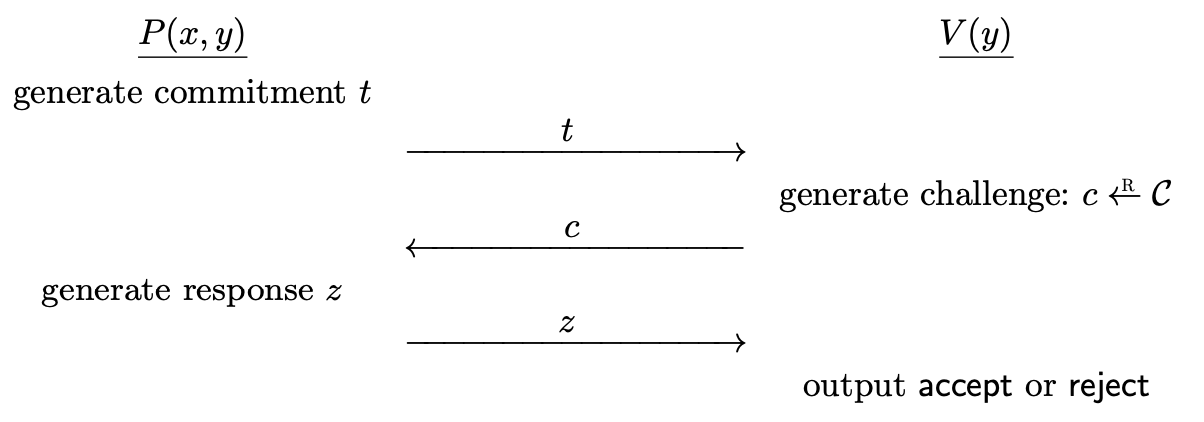
\includegraphics[width=0.75\linewidth]{figures/chapter19/fig5.png}
  \caption{Sigma协议的执行}
  \label{fig:19-5}
\end{figure}

图 \ref{fig:19-5} 展示了 Sigma 协议的执行流程。Sigma 协议的得名是因为这种协议中信息流的形状依稀让人想起希腊字母 $\Sigma$。

如定义所述,我们要求验证者的输出是陈述 $y$ 和对话 $(t,c,z)$ 的函数。当 $V$ 输出 $\mathsf{accept}$ 时,我们称对话 $(t,c,z)$ 是一个 $y$ \textbf{的接受对话 (accepting conversation for $y$)}。显然验证者与诚实的证明者之间只会产生接受对话;但当证明者不诚实或不遵循协议时,也有可能产生非接受对话。

在大多数 Sigma 协议的应用中,我们都会要求挑战空间的大小是超多项式的,为了简洁地表达该要求,我们有时也说协议需要\textbf{大的挑战空间}。

\begin{example}\label{exmp:19-1}
显然 Schnorr 识别协议 $(G,P,V)$ 中的算法 $(P,V)$ 是关系 $\mathcal{R}\subseteq\mathcal{X}×\mathcal{Y}$ 上的 Sigma 协议的一个特例,其中:
$$
\mathcal{X}=\mathbb{Z}_q,~~
\mathcal{Y}=\mathbb{G},~~
\mathcal{R}=\{(\alpha,u)\in\mathbb{Z}_q\times\mathbb{G}:g^\alpha=u\}
$$
挑战空间 $\mathcal{C}$ 是 $\mathbb{Z}_q$ 的一个子集。我们称 $(P,V)$ 为 \textbf{Schnorr的Sigma 协议 (Schnorr's Sigma protocol)}。

读者应该注意到,与识别协议不同的是,Sigma 协议本身并没有指定生成 $\mathcal{R}$ 中元素的算法。

还需要注意的是,关系 $\mathcal{R}$ 以群 $\mathbb{G}$ 作为参数,具体包括群 $\mathbb{G}$ 的阶 $q$ 和生成元 $g\in\mathbb{G}$。一般来说,我们允许用这种系统参数的方式来定义有效关系,这些参数在系统设置时产生,并公开给所有协议参与方。

Schnorr的Sigma 协议的陈述是一个群元素 $u\in\mathbb{G}$,而 $u$ 的见证是使得 $g^\alpha=u$ 成立的 $\alpha\in\mathbb{Z}_q$。因此每个陈述都对应着唯一的一个见证。一个 $u$ 的接受对话是一个形如 $(u_{\rm t},c,\alpha_{\rm z})$ 的三元组,其中 $u_{\rm t}\in\mathbb{G}$,$c\in\mathcal{C}$,$\alpha_{\rm z}\in\mathbb{Z}_q$,满足:
$$
g^{\alpha_{\rm z}}=u_{\rm t}\cdot u^c
$$

读者可能已经注意到,在 Schnorr 身份识别协议中,验证者 $P$ 只需要接受见证 $\alpha$ 作为输入,而不是像 Sigma 协议中所要求的见证-陈述对 $(\alpha,u)$。事实上,还有很多其他的 Sigma 协议的实例也同样不要求证明者在计算中显式地使用陈述。
\end{example}

\subsection{知识健全性}

接下来我们为 Sigma 协议定义一个关键的安全属性,称为\textbf{知识健全性 (knowledge soundness)}。

\begin{definition}[知识健全性]
令 $(P,V)$ 是一个关系 $\mathcal{R}\subseteq\mathcal{X}×\mathcal{Y}$ 上的 Sigma 协议,如果存在一个有效确定性算法 ${Ext}$(称为\textbf{见证提取器})具备下述属性:给定一个陈述 $y\in\mathcal{Y}$ 和 $y$ 的两个接受对话 $(t,c,z)$ 和 $(t,c',z')$ 作为输入,其中 $c\neq c'$,算法 ${Ext}$ 总是能输出 $x\in\mathcal{X}$ 使得 $(x,y)\in\mathcal{R}$,即 $x$ 是 $y$ 的一个见证;我们就称 Sigma 协议 $(P,V)$ 能够提供\textbf{知识健全性}。
\end{definition}

\begin{example}\label{exmp:19-2}
回顾例 \ref{exmp:19-1},我们很容易验证 Schnorr的Sigma 协议具备知识健全性。见证提取器 $\mathsf{Ext}$ 以 $u\in\mathbb{G}$ 为输入,并接受 $u$ 的两个接受对话 $(u_{\rm t},c,\alpha_{\rm z})$ 和 $(u_{\rm t},c',\alpha_{\rm z}')$,其中 $c\neq c'$。正如定理 \ref{theo:19-1} 的证明中所进行的操作,我们也可以从这两个接受对话中计算出相应的见证 $\alpha=\mathsf{Dlog}_gu$,其值为 ${\Delta\alpha}/{\Delta c}\in\mathbb{Z}_q$,其中 $\Delta\alpha:=\alpha_{\rm z}-\alpha_{\rm z}'$,$\Delta c:=c-c'$。
\end{example}

假设 $(P,V)$ 是关系 $\mathcal{R}\subseteq\mathcal{X}×\mathcal{Y}$ 上的 Sigma 协议。此外,假设 $(P,V)$ 提供知识健全性并且具有大的挑战空间。那么在某种意义上, $(P,V)$ 充当了一个\textbf{知识证明 (proof of knowledge)}。考虑任意一个证明者 $P^*$(甚至可能是一个潜在的``作弊"的验证者),使 $V$ 以不可忽略的概率接受一个陈述 $y$。那么$P^*$一定``知道" $y$ 的一个见证,方法如下:如定理 \ref{theo:19-1} 的证明中那样,我们可以回溯 $P^*$ 来得到 $y$ 的两个接受对话 $(t,c,z)$ 和 $(t,c',z')$,其中$c\neq c'$,然后使用见证提取器计算出见证 $x$。

更一般地说,当一个密码学家说 $P^*$ 一定``知道"一个陈述 $y$ 的见证时,她的意思是可以通过回溯从 $P^*$ 中提取出见证 $x$。虽然我们不会正式定义``知识证明"的概念,但我们将在一些应用中应用知识健全性。

\subsection{特殊诚实验证者零知识}

我们之前在 \ref{subsec:19-1-1}小节中介绍了用于身份认证协议的诚实验证者零知识(HVZK)的概念。我们现在可以很容易地将这个概念应用到 Sigma 协议的场景中。 

令 $(P,V)$ 是关系 $\mathcal{R}\subseteq\mathcal{X}×\mathcal{Y}$ 上的 Sigma 协议。直观上我们想表达的是,对于 $(x,y)\in\mathcal{R}$,$P(x,y)$ 和 $V(y)$ 之间的对话不应该透露任何关于见证 $x$ 的信息。下面我们将会严格定义这个直观上的概念,即我们可以在不了解见证 $x$ 的前提下有效模拟 $P(x,y)$ 和 $V(y)$ 之间的对话。然而,我们将增加一些额外的要求,这将简化一些构造和应用。

\begin{definition}[特殊诚实验证者零知识]
\label{def:19-5}
令 $(P,V)$ 是关系 $\mathcal{R}\subseteq\mathcal{X}×\mathcal{Y}$ 上的 Sigma 协议,其挑战空间为 $\mathcal{C}$。如果存在一个有效概率算法 ${Sim}$(称为\textbf{模拟器})以 $(y,c)\in\mathcal{Y}\times\mathcal{C}$ 为输入,并满足以下性质:
\begin{enumerate}
	\item 对于所有输入 $(y,c)\in\mathcal{Y}\times\mathcal{C}$ ,算法 ${Sim}$ 总是输出一个数对 $(t,z)$,使得 $(t,c,z)$ 是 $y$ 的一个接受对话;
	\item 对于任意 $(x,y)\in\mathcal{R}$,如果我们计算:
	$$
    c\overset{\rm R}\leftarrow\mathcal{C},~~
    (t,z)\overset{\rm R}\leftarrow {Sim}(y,c)
    $$
    则 $(t,c,z)$ 的分布与 $P(x,y)$ 与 $V(y)$ 之间对话记录的分布相同。
\end{enumerate}
则称 Sigma 协议 $(P,V)$ 是\textbf{特殊诚实验证者零知识(special honest verifier zero knowledge)}的,简称为\textbf{特殊 HVZK (special HVZK)} 的。
\end{definition}

读者有必要认识到这个定义的几个特点。首先,${Sim}$ 将挑战 $c$ 作为一个额外的输入。其次,要求即使陈述 $y$ 没有对应的见证,模拟器 ${Sim}$ 仍然能够产生一个接受对话。这两个特性是``特殊 HVZK"中``特殊"一词的原因。

\begin{example}
回到例 \ref{exmp:19-2},我们很容易验证 Schnorr的Sigma 协议是特殊 HVZK 的。事实上,我们可以将定理 \ref{theo:19-4} 的证明中的模拟器应用到这个场景中。对于输入 $u\in\mathbb{G}$ 和 $c\in\mathcal{C}$,模拟器计算:
$$
\alpha_{\rm z}\overset{\rm R}\leftarrow\mathbb{Z}_q,~~
u_{\rm t}\leftarrow{g^{\alpha_{\rm z}}}/{u^c}
$$
并输出 $(u_{\rm t},\alpha_{\rm z})$。读者可以自行验证该模拟器是否满足定义 \ref{def:19-5} 的所有要求。
\end{example}


\section{Sigma协议:范例}

到目前为止,我们所见过的唯一的 Sigma 协议是 Schnorr 协议,它允许一个证明者说服一个持怀疑态度的验证者,它``知道"一个给定群元素的离散对数,却不向验证者透露任何关于离散对数的信息。在本节中,我们将介绍另外几个 Sigma 协议的例子。这些例子不仅有助于充实 Sigma 协议的普遍理论,也有许多实际应用,其中的一些我们将在下面讨论。

\subsection{用于表示的 Okamoto 协议}\label{subsec:19-5-1}

令 $\mathbb{G}$ 是一个由 $g\in\mathbb{G}$ 生成的素阶 $q$ 的循环群,$h\in\mathbb{G}$ 是任意群元素。我们现在将 $h$ 看作是一个系统参数。所谓系统参数会在系统初始化时一次性生成,并对所有参与方公开。对于一个 $u\in\mathbb{G}$,如果给定 $g$ 和 $h$,可以使用一个数对 $(\alpha,\beta)\in\mathbb{Z}_q^2$ 来表示 $u$,方法是 $g^\alpha h^\beta=u$。

Okamoto 协议允许证明者说服持怀疑态度的验证者,它``知道"一个给定的 $u\in\mathbb{G}$ 的表示,但不需要向验证者透露任何有关该表示的具体信息。更确切地说,它是一个对于关系:
\begin{equation}\label{eq:19-11}
	\mathcal{R}=\bigg\lbrace
	\big((\alpha,\beta),u\big)\in\mathbb{Z}_q^2\times\mathbb{G}:g^\alpha h^\beta=u
	\bigg\rbrace
\end{equation}
的 Sigma 协议。陈述 $u\in\mathbb{G}$ 的一个见证 $u$ 是一个使得 $g^\alpha h^\beta=u$ 成立的数对 $(\alpha,\beta)\in\mathbb{Z}_q^2$,即 $u$ 的一个表示。因此,在这个例子中,每个陈述都对应着多个见证,准确的说是 $q$ 个见证。

通常假定 Okamoto 协议的挑战空间 $\mathcal{C}$ 是 $\mathbb{Z}_q$ 的一个子集。协议 $(P,V)$ 按如下方式运行,其中证明者 $P$ 由 $((\alpha,\beta),u)\in\mathcal{R}$ 初始化,验证者 $V$ 由 $u\in\mathbb{G}$ 初始化:
\begin{enumerate}
	\item $P$ 计算:
	$$
    \alpha_{\rm t}\overset{\rm R}\leftarrow\mathbb{Z}_q,~~
    \beta_{\rm t}\overset{\rm R}\leftarrow\mathbb{Z}_q,~~
    u_{\rm t}\leftarrow g^{\alpha_{\rm t}}h^{\beta_{\rm t}}
    $$
    并将承诺 $u_{\rm t}$ 发送给 $V$;
	\item $V$ 选取$c\overset{R}\leftarrow\mathcal{C}$,然后将挑战 $c$ 发送给 $P$;
	\item $P$ 计算:
	$$
    \alpha_{\rm z}\leftarrow\alpha_{\rm t}+\alpha c\in\mathbb{Z}_q,~~
    \beta_{\rm z}\leftarrow\beta_{\rm t}+\beta c\in\mathbb{Z}_q
    $$
    并将应答 $(\alpha_{\rm z}, \beta_{\rm z})$ 发送给 $V$;
	\item $V$ 检查$g^{\alpha_{\rm z}}h^{\beta_{\rm z}}\overset{?}=u_{\rm t}\cdot u^c$是否成立。如果是,$V$ 输出 $\mathsf{accept}$,否则 $V$ 输出 $\mathsf{reject}$。
\end{enumerate}
参见图 \ref{fig:19-6}。

\begin{figure}
  \centering
  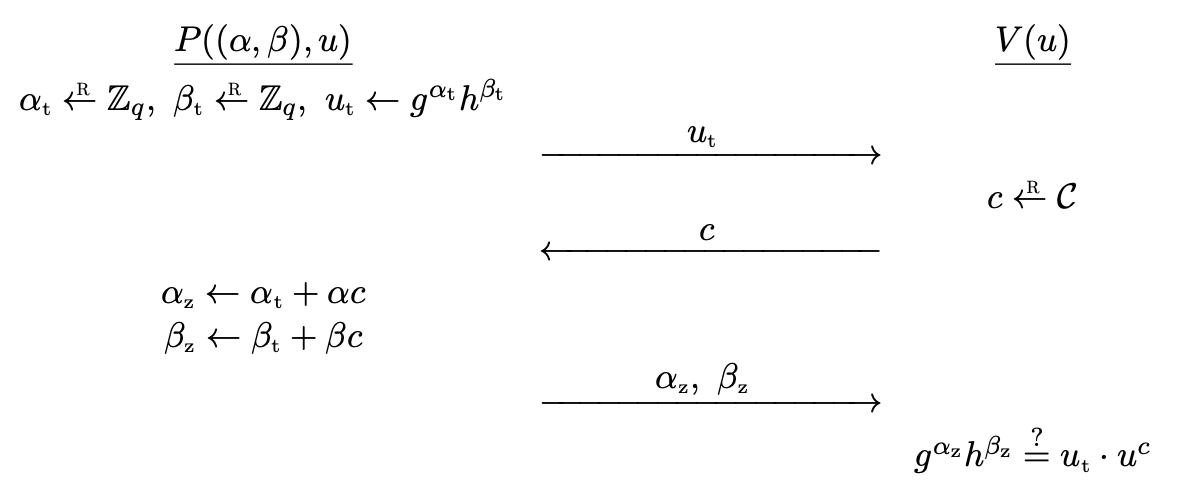
\includegraphics[width=0.75\linewidth]{figures/chapter19/fig6.png}
  \caption{Okamoto 协议}
  \label{fig:19-6}
\end{figure}

\begin{theorem}
Okamoto 协议是针对式 \ref{eq:19-11} 中定义的关系$\mathcal{R}$的一个 Sigma 协议。此外,Okamoto 协议提供知识健全性,且是特殊 HVZK 的。
\end{theorem}

\begin{proof}
显然,Okamoto 协议具有 Sigma 协议所要求的语法结构。陈述 $u\in\mathbb{G}$ 的一个接受对话形如:
$$
(u_{\rm t},c,(\alpha_{\rm z},\beta_{\rm z})) \text{~~s.t.~~} g^{\alpha_{\rm z}}h^{\beta_{\rm z}}=u_{\rm t}\cdot u^c
$$

\noindent
\emph{正确性.}
我们首先必须验证 Okamoto 协议是否满足基本的正确性要求,即诚实证明者和诚实验证者之间的交互总是能够产生一个接受对话。这很容易验证,因为如果:
$$
u_{\rm t}=g^{\alpha_{\rm t}}h^{\beta_{\rm t}},~~
\alpha_{\rm z}=\alpha_{\rm t}+\alpha c,~~
\beta_{\rm z}=\beta_{\rm t}+\beta c
$$
则我们有:
$$
g^{\alpha_{\rm z}}h^{\beta_{\rm z}}=
g^{\alpha_{\rm t}+\alpha c}h^{\beta_{\rm t}+\beta c}=
g^{\alpha_{\rm t}}h^{\beta_{\rm t}}\cdot(g^\alpha h^\beta)^c=
u_{\rm t}\cdot u^c
$$

\noindent
\emph{知识健全性.}
我们下面证明 Okamoto 协议提供知识健全性。假设我们现在有两个陈述 $u$ 的接受对话:
$$
(u_{\rm t},c,(\alpha_{\rm z},\beta_{\rm z})),~~
(u_{\rm t},c',(\alpha_{\rm z}',\beta_{\rm z}'))
$$
其中 $c\neq c'$。我们需要说明如何从这两个对话中有效提取 $u$ 的表示。这里的计算与 Schnorr 协议中的计算非常类似。注意到:
$$
g^{\alpha_{\rm z}}h^{\beta_{\rm z}}=u_{\rm t}\cdot u^c,~~
g^{\alpha_{\rm z}'}h^{\beta_{\rm z}'}=u_{\rm t}\cdot u^{c'}
$$
将第一个等式除以第二个等式,$u_{\rm t}$ 就被抵消了,于是我们有:
$$
g^{\Delta\alpha}h^{\Delta\beta}=u^{\Delta c},~~~~
\Delta\alpha:=\alpha_{\rm z}-\alpha_{\rm z}',~~
\Delta\beta:=\beta_{\rm z}-\beta_{\rm z}',~~
\Delta c:=c-c'
$$
因此,见证提取器可以用:
$$
\alpha\leftarrow{\Delta\alpha}/{c},~~
\beta\leftarrow{\Delta\beta}/{c}
$$
有效地计算出 $u$ 的一个表示 $(\alpha,\beta)\in\mathbb{Z}_q^2$。需要注意的是,由于 $c\neq c'$,$\Delta c$ 在 $\mathbb{Z}_q$ 中是可逆的。我们在这里利用了$q$是一个素数这个事实。

\vspace{5pt}

\noindent
\emph{特殊 HVZK.}
最后,我们通过给出一个模拟器来证明 Okamoto 协议是特殊 HVZK 的。这同样与 Schnorr 协议非常相似。对于输入 $u\in\mathbb{G}$ 和 $c\in\mathcal{C}$,模拟器计算:
$$
\alpha_{\rm z}\overset{\rm R}\leftarrow\mathbb{Z}_q,~~
\beta_{\rm z}\overset{\rm R}\leftarrow\mathbb{Z}_q,~~
u_{\rm t}\leftarrow{g^{\alpha_{\rm z}}h^{\beta_{\rm z}}}/{u^c}
$$
并输出 $(u_{\rm t},(\alpha_{\rm z},\beta_{\rm z}))$。可以发现,输出总是会产生一个符合要求的接受对话。

下面我们论证,当 $c\in\mathcal{C}$ 是随机选出的时候,模拟器在输入 $u,c$ 上的输出具有正确的分布。注意到在真实的对话中,$c$,$\alpha_{\rm z}$ 与 $\beta_{\rm z}$ 相互独立,其中 $c$ 在 $\mathcal{C}$ 上均匀分布,$\alpha_{\rm z}$ 和 $\beta_{\rm z}$ 在 $\mathbb{Z}_q$ 上均匀分布。此外,如果给定 $c$、$\alpha_{\rm z}$ 和 $\beta_{\rm z}$,$u_{\rm t}$ 的值由方程:

$$
g^{\alpha_{\rm z}}h^{\beta_{\rm z}}=u_{\rm t}\cdot u^c
$$
唯一决定。而这显然与模拟器的输出分布是一致的。
\end{proof}

\subsection{用于 DH 三元组的 Chaum-Pedersen 协议}\label{subsec:19-5-2}

Chaum-Pedersen 协议允许证明者在不向验证者透露任何其他信息的情况下,说服一个持怀疑态度的验证者相信一个给定的三元组是DH 三元组。

令 $\mathbb{G}$ 是一个 $q$ 阶循环群,其中 $q$ 是素数,$g\in\mathbb{G}$ 是生成元。回忆一下 10.5 节,对于 $\alpha,\beta,\gamma\in\mathbb{Z}_q$,如果 $\gamma=\alpha\beta$,我们就称元组 $(g^\alpha,g^\beta,g^\gamma)$ 为一个 DH 三元组 (DH-triple)。等价地,当且仅当存在 $\beta\in\mathbb{Z}_q$ 使得 $v=g^\beta$且$w=u^\beta$ 时,元组 $(u,v,w)$ 才是一个 DH 三元组。

Chaum-Pedersen 协议是关系:
\begin{equation}\label{eq:19-12}
\mathcal{R}:=\bigg\lbrace
\big(\beta, (u,v,w)\big)\in\mathbb{Z}_q\times\mathbb{G}^3:v=g^\beta, w=u^\beta
\bigg\rbrace
\end{equation}
上的 Sigma 协议。陈述 $(u,v,w)\in\mathbb{G}^3$ 的见证是使得 $v=g^\beta$ 且 $w=u^\beta$ 的一个 $\beta\in\mathbb{Z}_q$。因此,当且仅当陈述是一个 DH 三元组时,它才会存在一个见证。 与我们之前介绍的其它例子不同,在 Chaum-Pedersen 协议中,并非所有的陈述都必然存在见证。 

图 \ref{fig:19-7} 是 Chaum-Pedersen 协议 $(P,V)$ 的流程图,挑战空间 $\mathcal{C}$ 是 $\mathbb{Z}_q$ 的一个子集。

\begin{figure}
  \centering
  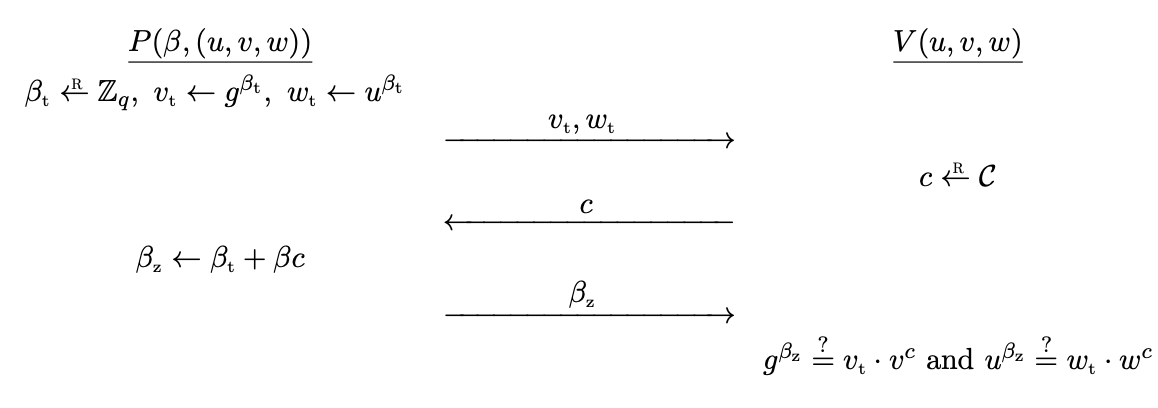
\includegraphics[width=0.75\linewidth]{figures/chapter19/fig7.png}
  \caption{Chaum-Pedersen 协议}
  \label{fig:19-7}
\end{figure}

\begin{theorem}
Chaum-Pedersen 协议是式 \ref{eq:19-12} 中定义的关系$\mathcal R$上的一个 Sigma 协议。此外,Chaum-Pedersen 协议提供知识健全性,且是特殊 HVZK 的。
\end{theorem}

\begin{proof}
显然,Chaum-Pedersen 协议具有 Sigma 协议所要求的语法结构。陈述 $(u,v,w)\in\mathbb{G}^3$ 的一个接受对话形如:
$$
((v_{\rm t},w_{\rm t}),c,\beta_{\rm z}) \text{~~s.t.~~} 
g^{\beta_{\rm z}}=v_{\rm t}\cdot v^c,~~
y^{\beta_{\rm z}}=w_{\rm t}\cdot w^c
$$
不难证明,一个诚实证明者与一个诚实验证者之间总是能够产生接受对话。

\noindent
\emph{知识健全性.}
假设我们有两个陈述 $(u,v,w)$ 的接受对话
$$
((v_{\rm t},w_{\rm t}),c,\beta_{\rm z}),~~
((v_{\rm t},w_{\rm t}),c',\beta_{\rm z}')
$$
其中 $c\neq c'$。不难发现
$$
\beta:={\Delta\beta}/{\Delta c}
$$
是陈述 $(u,v,w)\in\mathbb{G}^3$ 对应的见证,其中$\Delta\beta:=\beta_{\rm z}-\beta_{\rm z}'$,$\Delta c:=c-c'$。

\vspace{5pt}

\noindent
\emph{特殊 HVZK.}
对于输入 $(u,v,w)\in\mathbb{G}^3$ 和 $c\in\mathcal{C}$ 时,模拟器计算:
$$
\beta_{\rm z}\overset{\rm R}\leftarrow\mathbb{Z}_q,~~
v_{\rm t}\leftarrow{g^{\beta_{\rm z}}}/{v^c},~~
w_{\rm t}\leftarrow{u^{\beta_{\rm z}}}/{w^c}
$$
并输出 $((v_{\rm t},w_{\rm t}),c,\beta_{\rm z})$。可以发现,输出总是会产生一个符合要求的接受对话。

下面我们论证,当 $c\in\mathcal{C}$ 是随机选出的时候,模拟器在输入 $((u,v,w),c)$ 上的输出具有正确的分布。注意到在真实的对话中,$c$ 和 $\beta_{\rm z}$ 相互独立,其中 $c$ 在 $\mathcal{C}$ 上均匀分布,$\beta_{\rm z}$ 在 $\mathbb{Z}_q$ 上均匀分布。此外,如果给定 $c$ 和 $\beta_{\rm z}$,$v_{\rm t}$ 和 $w_{\rm t}$ 的值由
$$
g^{\beta_{\rm z}}=v_{\rm t}\cdot v^c, ~~
u^{\beta_{\rm z}} =w_{\rm t}\cdot w^c
$$
唯一决定。而这显然与模拟器的输出分布是一致的。
\end{proof}

\subsection{用于任意线性关系的 Sigma 协议}\label{subsec:19-5-3}

读者可能已经注意到 Schnorr、Okamoto 和 Chaum-Pedersen 协议之间的某些相似之处。事实上,它们都是用于证明一组元素之间线性关系的通用 Sigma 协议的特例。

与之前一样,令 $\mathbb{G}$ 是一个 $q$ 阶循环群,其中 $q$ 是素数,$g\in\mathbb{G}$ 是生成元。考察形如:
\begin{equation}\label{eq:19-13}
\phi(x_1,\dots,x_n):=
\left\{
~u_1=\prod^n_{j=1}g_{1j}^{x_j} ~~\land~~\cdots~~\land~~ u_m=\prod^n_{j=1}g_{mj}^{x_j}~
\right\}
\end{equation}
的布尔表达式 $\phi$。其中所有的 $g_{ij}$ 和 $u_i$ 都是 $\mathbb{G}$ 中的元素,这些元素中的有些可以是系统参数甚至是常数,有些是表达式特有的。$\phi$ 中的 $x_i$ 是公式的变量。当我们给 $x_1,\dots,x_n$ 赋 $\mathbb{Z}_q$ 中的值时,如果式 \ref{eq:19-13} 中的所有等式都成立,$\phi$ 就会输出 true。

对于这类公式的集合 $\mathcal{F}$,我们可以定义关系:
\begin{equation}\label{eq:19-14}
\mathcal{R}:=
\bigg\lbrace
\Big(
(\alpha_1,\dots,\alpha_n),\phi
\Big)
\in\mathbb{Z}_q^n\times\mathcal{F}: ~\phi(x_1,\dots,x_n)={\rm{true}}~
\bigg\rbrace
\end{equation}
因此,陈述是一个表达式 $\phi\in\mathcal{F}$,$\phi$ 的见证是能使得表达式 $\phi$ 输出 true 的 $x_1,\dots,x_n$ 的一组赋值 $(\alpha_1,\dots,\alpha_n)\in\mathbb{Z}_q^n$。我们之所以称其为``线性"关系集,是因为如果我们取离散对数,式 \ref{eq:19-13} 就可以改写为如下的线性方程组:
$$
{\rm\mathsf{Dlog}}_g(u_j)=\sum_{j=1}^nx_i\cdot {\rm\mathsf{Dlog}}_g(g_{ij})~~~~(i=1,2,\dots,m)
$$
而见证就是上述线性方程组的一组解。

\begin{figure}
  \centering
  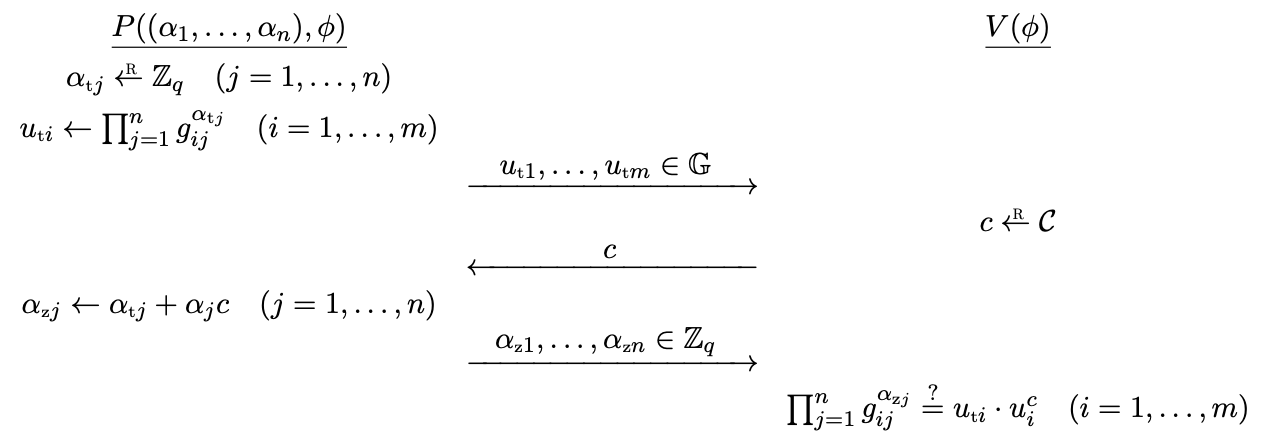
\includegraphics[width=0.85\linewidth]{figures/chapter19/fig8.png}
  \caption{通用线性协议}
  \label{fig:19-8}
\end{figure}

图 \ref{fig:19-8} 展示了关系 $\mathcal{R}$ 上的\textbf{通用线性协议 (generic linear protocol)} $(P,V)$。证明者拥有 $\phi$ 和见证 $(\alpha_1,\dots,\alpha_n)\in\mathbb{Z}_q^n$,挑战空间 $\mathcal{C}$ 是 $\mathbb{Z}_q$ 的一个子集。这样,到目前为止我们所介绍的所有 Sigma 协议都是这个通用线性协议的特例:
\begin{itemize}
	\item Schnorr 协议对应着 $\phi_1(x):=\{u=g^x\}$ 的情况。
	\item Okamoto 协议对应着 $\phi_2(x,y):=\{u=g^xh^y\}$ 的情况。
	\item Chaum-Pedersen 协议对应着 $\phi_3(x):=\{v=g^x\land w=u^x\}$ 的情况。
\end{itemize}

我们可以通过模仿Schnorr、Okamoto和Chaum-Pedersen的相应定理的证明来证明以下定理。我们把它作为一个练习留给读者。

\begin{theorem}\label{theo:19-11}
图 \ref{fig:19-8} 所描述的通用线性协议是式 \ref{eq:19-14} 中定义的关系 $\mathcal R$ 上的一个 Sigma 协议。此外,该协议提供知识健全性,且是特殊 HVZK 的。
\end{theorem}

我们还可以进一步泛化这个通用线性协议,方法是允许式 \ref{eq:19-13} 中的各个方程定义在不同的群上。唯一的要求是所有群都有相同的素阶 $q$。这种更通用的线性协议的典型出现场景是有两类方程,其中一类定义在密码学所感兴趣的群 $\mathbb{G}$ 上,群的阶为素数 $q$;另一类定义在 $\mathbb{Z}_q$ 上,其形式为 $\kappa_i=\sum_{j=1}^n\lambda_{ij}x_j$,其中 $\kappa_i$ 和 $\lambda_{ij}$ 是 $\mathbb{Z}_q$ 中的元素。

\subsection{一种用于同态原像的 Sigma 协议}

到目前为止我们介绍的所有 Sigma 协议,包括通用线性协议,都可以用群同态的语言来更清楚、更简洁地描述。令 $\mathbb{H}_1$ 和 $\mathbb{H}_2$ 是两个阶已知的有限阿贝尔群,$\psi:\mathbb{H}_1\to\mathbb{H}_2$ 是一个群同态。我们将群 $\mathbb{H}_1$ 中的运算表示为加法形式,将群 $\mathbb{H}_2$ 中的运算表示为乘法形式。

\begin{figure}
  \centering
  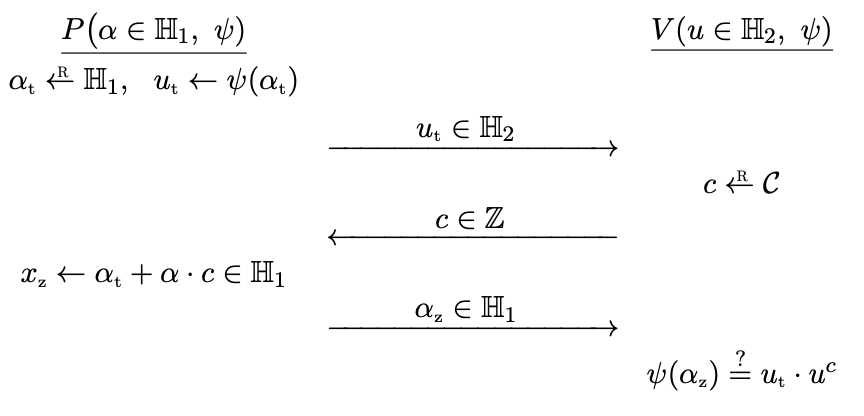
\includegraphics[width=0.6\linewidth]{figures/chapter19/fig9.png}
  \caption{用于同态原像的 Sigma 协议}
  \label{fig:19-9}
\end{figure}

令 $u\in\mathbb{H}_2$。图 \ref{fig:19-9} 展示了一个 Sigma 协议,它允许证明者说服验证者它``知道" $u$ 在 $\psi$ 下的原像。具体地,该协议是关系:
\begin{equation}\label{eq:19-15}
\mathcal{R}:=\bigg\lbrace
\Big(\alpha,(u,\psi)\Big)\in\mathbb{H}_1\times(\mathbb{H}_1\times\mathcal{F}):\psi(\alpha)=u
\bigg\rbrace
\end{equation}
上的一个 Sigma 协议。其中 $\alpha\in\mathbb{H}_1$ 是 $u\in\mathbb{H}_2$ 在 $\psi$ 下的原像。图 \ref{fig:19-9} 中的证明者持有见证 $\alpha\in\mathbb{H}_1$,验证者持有像 $u\in\mathbb{H}_2$,双方共有 $(\mathbb{H}_1,\mathbb{H}_2,\psi)$。挑战空间 $\mathcal{C}$ 为 $\{0,1,\dots,N-1\}\subseteq\mathbb{Z}$,其中 $N$ 为特定整数。

下面让我们看看这个协议是如何包含到目前为止所有的 Sigma 协议实例的。令 $\mathbb{G}$ 是一个素阶 $q$ 的群,且有生成元 $g,h,u\in\mathbb{G}$:
\begin{itemize}
	\item Okamoto 协议对应着 $\mathbb{H}_1:=\mathbb{Z}_q^2$,$\mathbb{H}_2:=\mathbb{G}$ 且 $\psi_1(x,y):=g^xh^y$ 的特殊情况。
	\item Chaum-Pedersen 协议对应着
	$$\mathbb{H}_1:=\mathbb{Z}_q,~~\mathbb{H}_2:=\mathbb{G}^2, ~~\psi_2(x):=(g^x,u^x)$$
	的特殊情况。我们甚至可以令 $\mathbb{H}_2=\mathbb{G}_1\times\mathbb{G}_2$,其中 $g\in\mathbb{G}_1$,$u\in\mathbb{G}_2$,并且 $|\mathbb{G}_1|=|\mathbb{G}_2|$。那么对于一个给定的 $(v,w)\in\mathbb{G}_1\times\mathbb{G}_2$,提供$(v, w)$ 在 $\psi_2$ 上的一个原像与计算群 $\mathbb{G}_1$ 和 $\mathbb{G}_2$ 上的离散对数问题 $\mathsf{Dlog}_g(v)=\mathsf{Dlog}_u(w)$ 等价。
	\item 图 \ref{fig:19-8} 中的通用线性协议对应着
	$$
    \mathbb{H}_1:=(\mathbb{Z}_q)^n,~~
    \mathbb{H}_2:=\mathbb{G}^m,~~
    \psi_3(x_1,\dots,x_n):=
    \left(
    ~\prod_{j=1}^ng_{1j}^{x_j},~\dots,~\prod_{j=1}^ng_{mj}^{x_j}~
    \right)
    $$
    的特殊情况。其中,对于所有的$i=1,\dots,m$和$j=1,\dots,n$,都有$g_{ij}\in\mathbb{G}$。
\end{itemize}
我们可以很容易地验证 $\psi_1,\psi_2,\psi_3$ 的映射都是群同态的。通过在图 \ref{fig:19-9} 中的协议使用这些同态映射,我们可以得到本节中介绍的所有 Sigma 协议实例。

\begin{theorem}\label{theo:19-12}
图 \ref{fig:19-9} 中的协议是式 \ref{eq:19-15} 中定义的关系 $\mathcal R$ 上的一个 Sigma 协议。此外,该协议是特殊 HVZK 的,而且只要 $|\mathbb{H}_1|\times|\mathbb{H}_2|$ 的最小素因子至少是 $|\mathcal{C}|$,该协议就提供知识健全性。
\end{theorem}

定理 \ref{theo:19-12} 的证明完全模仿了 Schnorr 协议相应定理的证明。对 $|\mathbb{H}_1|\times|\mathbb{H}_2|$ 的最小素因子的下限要求,是为了确保见证提取器可以从两个接受对话 $(u_{\rm t},c,\alpha_{\rm z})$ 和 $(u_{\rm t},c',\alpha_{\rm z}')$ 中获得一个映射 $\psi$ 的原像。就如同在 Schnorr 协议中的见证提取器中那样,我们可以得到$\psi(\Delta\alpha)=u^{\Delta c}$,其中$\Delta\alpha:=(\alpha_z-\alpha_z')\in\mathbb{H}_1$,$\Delta c=(c-c')\in\mathbb{Z}$。限制 $|\mathbb{H}_1|$ 和 $|\mathbb{H}_2|$ 素因子的下界是为了确保(1)我们可以在 $\mathbb{H}_1$ 中用 $\Delta c$ 除以 $\Delta\alpha$,并且(2)我们可以在等式两边同时升幂 $((\Delta c)^{-1}\mod |\mathbb{H}_2|)\in\mathbb{Z}$,以求得等式右项的 $\Delta c$ 次方根。然后,我们就可以得到$\psi({\Delta\alpha}/{\Delta c})=u$,因此 ${\Delta\alpha}/{\Delta c}\in\mathbb{H}_1$ 就是 $u\in\mathbb{H}_2$ 在映射 $\psi$ 下的原像。

\subsection{一种用于 RSA 的 Sigma 协议}\label{subsec:19-5-5}

为了避免读者认为 Sigma 协议只适用于与离散对数有关的问题,我们下面介绍一个与 RSA 有关的协议。

令 $(n,e)$ 是一个 RSA 公钥,$e$ 是一个素数。我们将 $(n,e)$ 视为一个系统参数。Guillou-Quisquater (GQ) 协议允许证明者说服持怀疑态度的验证者,它``知道" $y\in\mathbb{Z}_n^*$ 的一个 $e$ 次方根,而不透露任何其他信息。更确切地说,GQ 协议是关系:
\begin{equation}\label{eq:19-16}
\mathcal{R}=
\bigg\lbrace
(x,y)\in\mathbb{Z}_n^*\times\mathbb{Z}_n^*:x^e=y
\bigg\rbrace
\end{equation}
上的一个 Sigma 协议。陈述 $y\in\mathbb{Z}_n^*$ 的见证是 $x\in\mathbb{Z}_n^*$,满足 $x^e=y$。由于 $(n,e)$ 是一个 RSA 公钥,因此由 $x\in\mathbb{Z}_n^*$ 到 $y=x^e\in\mathbb{Z}_n^*$ 的映射是一个双射。因此每个陈述都对应着唯一的见证。

\begin{figure}
  \centering
  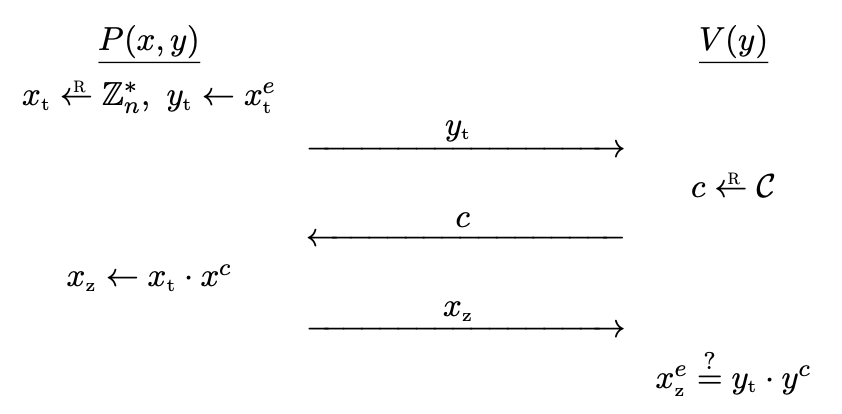
\includegraphics[width=0.6\linewidth]{figures/chapter19/fig10.png}
  \caption{Guillou-Quisquater 协议}
  \label{fig:19-10}
\end{figure}


图 \ref{fig:19-10} 展示了 GQ 协议 $(P,V)$ 的工作流程。其挑战空间 $\mathcal{C}$ 是 $\{0,\dots,e-1\}$ 的一个子集。需要注意的是,当 $e$ 很小时,挑战空间也很小。如果需要,我们可以用练习 19.5 中介绍的方法将其扩大。然而在使用该协议时,我们通常会将 $e$ 设定为一个大素数来确保挑战空间是足够大的。

图 \ref{fig:19-10} 中的 GQ 协议也是图 \ref{fig:19-9} 中展示的用于同态原像的 Sigma 协议的一个特例。此时群同态是 $\psi:\mathbb{Z}_n^*\to\mathbb{Z}_n^*$,定义为 $\psi(x)=x^e$。然而,我们无法像定理 \ref{theo:19-12} 那样证明 GO 协议提供知识健全性,因为群 $\mathbb{Z}_n^*$ 的阶是未知的。相反地,我们必须对这些属性进行单独证明。我们有下面的定理。

\begin{theorem}
GQ协议是式 \ref{eq:19-16} 中定义的关系$\mathcal R$上的一个Sigma协议。此外,它提供知识健全性,并且是特殊HVZK的。
\end{theorem}

\begin{proof}
$y$ 的一个接受对话形如 $(x_{\rm t},c,x_{\rm z})$,其中 $x^e_{\rm z}=y_{\rm t}\cdot y^c$。读者很容易验证基本的正确性要求,即一个诚实证明者和一个诚实验证者之间的交互总是会产生一个接受对话。

\vspace{5pt}

\noindent
\emph{知识健全性.}
下面我们将证明 GQ 协议具备知识健全性。假设我们有两个陈述 $y$ 的接受对话 $(x_{\rm t},c,x_{\rm z})$ 和 $(x_{\rm t},c',x_{\rm z}')$,其中 $c\neq c'$。我们必须证明能够有效计算出 $y$ 的 $e$ 次方根。观察到:
$$
x^e_{\rm z}=y_{\rm t}\cdot y^c,~~
(x_{\rm z}')^e=y_{\rm t}\cdot y^{c'}
$$
将第一个方程除以第二个方程,可以得到:
$$
(\Delta x)^e=y^{\Delta c}
$$
其中:$\Delta x:={x_{\rm z}}/{x_{\rm z}'}$,$\Delta c:=c-c'$。由于 $c\neq c'$,且 $c$ 和 $c'$ 都属于区间 $\{0,\dots,e-1\}$,因此有 $0<|\Delta c|<e$,所以 $e\nmid\Delta c$。此外由于 $e$ 是素数,所以 $\gcd(e,\Delta c)=1$。因此当给定 $e$,$f:=\Delta c$,$w:=\Delta x$ 时,我们可以利用定理 10.6 求得 $y$ 的 $e$ 次方根。

读者应该注意到,这里给出的从两个接受对话中计算 RSA 逆变换的技术与定理 10.7 的证明中使用的方法基本相同。事实上,这两个接受对话制造了哈希函数 $H_{\rm rsa}(a,b)=a^ey^b$ 上的一次碰撞 $((x_{\rm z},-c\mod e),(x_{\rm z}',-c'\mod e))$。

\vspace{5pt}

\noindent
\emph{特殊 HVZK.}
最后,我们通过给出一个模拟器来证明 GQ 协议是特殊 HVZK 的。对于输入 $y\in\mathbb{Z}_n^*$ 和 $c\in\mathcal{C}$,模拟器计算:
$$
x_{\rm z}\overset{\rm R}\leftarrow\mathbb{Z}_n^*,~~
y_{\rm t}\leftarrow{x_{\rm z}^e}/{y^c}
$$
并输出 $(y_{\rm t},x_{\rm z})$。注意到在真实的对话中,$c$ 和 $x_{\rm z}$ 是相互独立的,$c$ 在 $\mathcal{C}$ 上均匀分布,$x_z$ 在 $\mathbb{Z}_n^*$ 上均匀分布。此外,如果给定 $c$ 和 $x_z$,$y_t$ 的值由方程$x^e_{\rm z}=y_{\rm t}\cdot y^c$唯一决定。而这显然与模拟器的输出分布是一致的。
\end{proof}
\section{基于Sigma协议的身份识别和签名}\label{sec:19-6}

通过模仿 Schnorr 构造,我们很容易将任何 Sigma 协议转换成相应的识别方案和签名方案。

假设我们有一个关系 $\mathcal{R}\subseteq\mathcal{X}×\mathcal{Y}$ 上的 Sigma 协议 $(P,V)$。除了算法 $P$ 和 $V$ 之外,我们还需要一个 $\mathcal{R}$ \textbf{上的密钥生成算法}。它是一个概率算法 $G$,生成一个公私钥对 $(pk,sk)$,其中 $pk=y$,$sk=(x,y)$,$(x,y)\in\mathcal{R}$。

为了得到安全的识别和签名方案,我们需要以下的``单向性"特征:给定 $G$ 输出的公钥 $pk=y\in\mathcal{Y}$,应该很难计算出一个 $\hat x\in\mathcal{X}$ 满足 $(\hat x,y)\in\mathcal{R}$。我们用下面的攻击游戏来更加精准地描述这个概念。

\begin{game}[单向密钥生成]\label{game:19-2}
令 $G$ 是 $\mathcal{R}\subseteq\mathcal{X}×\mathcal{Y}$ 上的一个密钥生成算法。对于一个给定对手 $\mathcal{A}$,攻击游戏按如下方式运行:
\begin{itemize}
	\item 挑战者运行 $(pk,sk)\overset{\rm R}\leftarrow G()$,并将 $pk=y$ 发送给 $\mathcal{A}$;
	\item $\mathcal{A}$ 输出 $\hat x\in\mathcal{X}$。
\end{itemize}
如果 $(\hat x,y)\in\mathcal{R}$,我们就称对手赢得了攻击游戏。我们将 $\mathcal{A}$ 相对于 $\mathbb{G}$ 的优势定义为 ${\rm OW\mathsf{adv}}[\mathcal{A},\mathbb{G}]$,其值为 $\mathcal{A}$ 赢得游戏的概率。
\end{game}

\begin{definition}
如果对于所有有效对手 $\mathcal{A}$,${\rm OW\mathsf{adv}}[\mathcal{A},\mathbb{G}]$ 的值都是可忽略不计的,我们就称密钥生成算法 $G$ 是\textbf{单向的}。
\end{definition}

\begin{example}\label{exmp:19-4}
对于例 \ref{exmp:19-1} 介绍的 Schnorr的Sigma 协议,最自然的密钥生成算法是计算 $\alpha\overset{\rm R}\leftarrow\mathbb{Z}_q$ 和 $u\leftarrow g^\alpha\in\mathbb{G}$,并输出 $pk:=u$ 和 $sk:=(\alpha,u)$。在离散对数假设下,这种密钥生成算法显然是单向的。
\end{example}

\begin{example}\label{exmp:19-5}
考虑 \ref{subsec:19-5-5} 小节介绍的 GQ 协议,其中 RSA 公钥 $(n, e)$ 被视为一个系统参数。最自然的密钥生成算法是计算 $x\overset{\rm R}\leftarrow\mathbb{Z}_n^*$ 和 $y\leftarrow x^e\in\mathbb{Z}_n^*$,并输出 $pk:=y$ 和 $sk:=(x,y)$。在 RSA 假设下,这种密钥生成算法显然也是单向的(见定理10.5)。
\end{example}

一个含有密钥生成算法 $G$ 的 Sigma 协议 $(P,V)$ 能够提供一个身份识别方案 $(G,P,V)$。接下来的两个定理将证明它对窃听攻击是安全的。

\begin{theorem}
令 $(P,V)$ 是一个具有大挑战空间的有效关系 $\mathcal{R}$ 上的 Sigma 协议。令 $G$ 是$\mathcal{R}$ 的一个密钥生成算法。如果 $(P,V)$ 提供知识健全性,并且 $G$ 是单向的,那么身份识别方案 $\mathcal{I}:=(G,P,V)$ 对于直接攻击是安全的。

\begin{quote}
特别地,假设 $\mathcal{A}$ 是一个有效冒充对手,他通过攻击游戏 \ref{game:18-1} 中的直接攻击来攻击 $\mathcal{I}$,其优势为 $\epsilon:=\rm{ID1\mathsf{adv}}[\mathcal{A},\mathcal{I}]$。则必然存在一个有效对手 $\mathcal{B}$如攻击游戏 \ref{game:19-2} 那样攻击 $G$,其运行时间大约是 $\mathcal{A}$ 的两倍,其优势 $\epsilon':={\rm OW\mathsf{adv}}[\mathcal{A},\mathbb{G}]$,那么:
\end{quote}
\begin{equation}\label{eq:19-17}
\epsilon'\geq \epsilon^2-\frac{\epsilon}{N}
\end{equation}
\begin{quote}
其中 $N$ 是挑战空间的大小,这意味着:
\end{quote}
\begin{equation}\label{eq:19-18}
\epsilon\leq\frac{1}{N}+\sqrt{\epsilon'}
\end{equation}
\end{theorem}

\begin{proof}
我们可以模仿定理 \ref{theo:19-1} 的证明。利用冒充对手 $\mathcal{A}$,我们可以使用下述方法建立一个打破 $G$ 的单向性的对手 $\mathcal{B}$。对手 $\mathcal{B}$ 从其挑战者那里得到一个公钥 $pk = y$,而我们的目标是让 $\mathcal{B}$ 在 $\mathcal{A}$ 的帮助下计算出一个满足 $(\hat x,y)\in\mathcal{R}$的$\hat x$。$\mathcal{B}$ 的行为可以分为两个阶段。

在第一阶段,$\mathcal{B}$ 扮演 $\mathcal{A}$ 的挑战者的角色,给 $\mathcal{A}$ 提供值 $pk=y$ 作为验证公钥。使用与定理 \ref{theo:19-1} 的证明中相同的回溯方法,对手 $\mathcal{B}$ 可以以至少 $\epsilon^2-{\epsilon}/{N}$ 的概率获得 $y$ 的两个接受对话 $(t,c,z)$ 和 $(t,c',z')$,其中 $c\neq c'$。更具体地说,$\mathcal{B}$ 等待来自 $\mathcal{A}$ 的承诺 $t$,接着向 $\mathcal{A}$ 发送一个随机挑战 $c$,并等待 $\mathcal{A}$ 的应答 $z$。在此之后,$\mathcal{B}$ 将 $\mathcal{A}$ 的内部状态回溯到它产生 $t$ 的那一时刻,然后向 $\mathcal{A}$ 发送另一个随机挑战 $c'$,并等待 $\mathcal{A}$ 的应答 $z'$。根据回溯引理(引理\ref{theo:19-2}),这个过程将以至少 $\epsilon^2-{\epsilon}/{N}$ 的概率产生两个接受对话。

在计算的第二阶段,$\mathcal{B}$ 将这两个接受对话送入见证提取器(由知识健全性保证存在),以为 $y$ 提取一个见证 $\hat x$。

这样我们就证明了式 \ref{eq:19-17},而式 \ref{eq:19-18}可以通过与定理 \ref{theo:19-1} 相同的方式得到。
\end{proof}

定理 \ref{theo:19-3} 显然适用于从特殊 HVZK 的 Sigma 协议衍生出来的身份识别协议:

\begin{theorem}\label{theo:19-15}
令 $(P,V)$ 是一个有效关系 $\mathcal{R}$ 上的 Sigma 协议。令 $G$ $\mathcal{R}$ 的一个密钥生成算法。如果一个身份识别协议 $\mathcal{I}=(G,P,V)$ 对于直接攻击是安全的,且$(P,V)$是特殊 HVZK 的,那么 $\mathcal{I}$ 对于窃听攻击也是安全的。
\begin{quote}
特别地,对于每一个通过攻击游戏 18.2 中的窃听攻击来攻击 $\mathcal{I}$ 的冒充对手 $\mathcal{A}$,必然存在一个通过攻击游戏 \ref{game:18-1} 中的直接攻击来攻击 $\mathcal{I}$ 的对手 $\mathcal{B}$,其中 $\mathcal{B}$ 是 $\mathcal{A}$ 的一个基本包装器,使得:
\end{quote}
$$
{\rm ID2\mathsf{adv}}[\mathcal{A},\mathcal{I}]=
{\rm ID1\mathsf{adv}}[\mathcal{B},\mathcal{I}]
$$
\end{theorem}

\begin{example}\label{exmp:19-6}
如果我们用例 \ref{exmp:19-5} 中的密钥生成算法 $G$ 来增强 GQ 协议 $(P,V)$,我们就能够得到识别方案 $\mathcal{I}_{\rm GQ}=(G,P,V)$,只要挑战空间足够大,该识别方案在 RSA 假设下对窃听攻击就是安全的。
\end{example}

\subsection{用于签名的 Fiat-Shamir 启发式算法}\label{subsec:19-6-1}

使用 \ref{sec:19-2} 节中介绍的技术,我们就可以将 Sigma 协议转换为签名方案。这个普适的技术最早由 Fiat 和 Shamir 提出,它包含如下几个部分:
\begin{itemize}
	\item 一个关系 $\mathcal{R}\subseteq\mathcal{X}×\mathcal{Y}$ 上的 Sigma 协议 $(P,V)$。我们假设对话形如 $(t,c,z)$,其中 $t\in\mathcal{T}$,$c\in\mathcal{C}$,$z\in\mathcal{Z}$;
	\item 一个关系 $\mathcal{R}$ 的密钥生成算法 $G$;
	\item 一个哈希函数 $H:\mathcal{M}\times\mathcal{T}\to\mathcal{C}$,它被建模为一个随机预言机。集合 $\mathcal{M}$ 也同样是签名方案的消息空间。
\end{itemize}

由 $G$ 和 $(P, V)$ 派生出的\textbf{Fiat-Shamir 签名方案}的工作原理如下:
\begin{itemize}
	\item 密钥生成算法为 $G$,所以公钥形如 $pk=y$, 其中$y\in\mathcal{Y}$,私钥形如 $sk=(x,y)\in\mathcal{R}$。
	\item 使用私钥 $sk = (x, y)$ 对消息 $m\in\mathcal{M}$ 进行签名,签名算法运行如下:
	\begin{itemize}
		\item 运行验证者 $P(x,y)$ 并获得一个承诺 $t\in\mathcal{T}$;
		\item 计算挑战 $c\leftarrow H(m,t)$;
		\item 最后,将 $c$ 发送给证明者并得到一个应答 $z$,然后输出签名 $\sigma:=(t,z)\in\mathcal{T}\times\mathcal{Z}$。
	\end{itemize}
	\item 为了使用公钥 $pk=y$ 验证对消息 $m\in\mathcal{M}$ 的签名 $\sigma=(t,z)\in\mathcal{T}\times\mathcal{Z}$,验证算法计算 $c\leftarrow H(m,t)$,并检查 $(t,c,z)$ 是否是 $y$ 的接受对话。
\end{itemize}

正如我们对 Schnorr 协议所做的那样,我们下面会证明如果对应的识别方案 $(G,P,V)$ 对窃听攻击是安全的,那么 Fiat-Shamir 签名方案在随机预言机模型下是安全的。然而,我们还需要一个技术上的假设,基本上所有我们感兴趣的 Sigma 协议都满足这个假设。

\begin{definition}[不可预测承诺]\label{def:19-7}
令 $(P,V)$ 是关系 $\mathcal{R}\subseteq\mathcal{X}×\mathcal{Y}$ 上的 Sigma 协议,并假定所有对话 $(t,c,z)$ 都位于 $\mathcal{T}\times\mathcal{C}\times\mathcal{Z}$ 中。如果对于任意 $(x,y)$ 和 $\hat t\in\mathcal{T}$,$P(x,y)$ 和 $V(y)$ 之间的交互会以最多 $\delta$ 的概率产生一个对话 $(t,c,z)$ 满足 $t=\hat t$,则称 $(P,V)$ 有 \textbf{$\delta$-不可预测承诺 ($\delta$-unpredictable commitments)}。如果 $(P,V)$ 有 $\delta$-不可预测承诺,且 $\delta$ 的值不可忽略不计,我们就称 $(P,V)$ 有不可预测承诺。
\end{definition}

\begin{theorem}\label{theo:19-16}
如果 $H$ 被建模为一个随机预言机,身份识别方案 $\mathcal{I}=(G,P,V)$ 对窃听攻击是安全的,并且 $(P,V)$ 有不可预测承诺,那么从 $G$ 和 $(P, V)$ 派生出的 Fiat-Shamir 签名方案 $\mathcal{S}$ 是安全的。
\begin{quote}
	特别地,令 $\mathcal{A}$ 是一个像在攻击游戏 13.1 的随机预言机版本中一样的攻击 $\mathcal{S}$ 的对手。此外,假设 $\mathcal{A}$ 最多可以发起 $Q_{\rm s}$ 次签名查询和 $Q_{\rm ro}$ 次随机预言机查询,并且 $(P, V)$ 有 $\delta$-不可预测承诺。那么必然存在一个 $(Q_{\rm ro}+1)$ 次重复冒充攻击对手 $\mathcal{B}$,它能够通过攻击游戏 \ref{game:19-1} 中的窃听攻击来攻击 $\mathcal{I}$,其中 $\mathcal{B}$ 是 $\mathcal{A}$ 的一个基本包装器,使得:
\end{quote}
$$
{\rm SIG^{ro}\mathsf{adv}}[\mathcal{A},\mathcal{S}]\leq Q_{\rm s}(Q_{\rm s}+Q_{\rm ro}+1)\delta+{\rm rID2\mathsf{adv}}[\mathcal{B},\mathcal{I},Q_{\rm ro}+1]
$$
\end{theorem}

这个定理的证明与定理 \ref{theo:19-7} 的证明几乎相同,读者可以尝试自己证明该定理。

把以上结论结合起来,假设我们从一个 Sigma 协议 $(P, V)$ 开始,该协议是特殊 HVZK 的,并且它能提供知识健全性。此外,假设 $(P, V)$ 有不可预测承诺和一个大的挑战空间。那么,如果我们把 $(P, V)$ 和一个单向密钥生成算法 $G$ 结合起来,就可以利用 Fiat-Shamir 签名构造法基于一个随机预言机 $H$ 构建一个安全的签名方案。事实上,Schnorr 签名方案就是这个结构的一个特例。

就像我们对 Schnorr 签名所做的那样,我们也可以使用引理 \ref{theo:19-6} 将问题从 $r$ 次重复冒充规约到 $1$ 次冒充。但是更严格的规约也是有可能的,事实上引理 \ref{theo:19-8} 的证明在这里也是成立的,基本上不需要更改太多内容:

\begin{lemma}\label{theo:19-17}
令 $(P,V)$ 是一个关系 $\mathcal{R}\subseteq\mathcal{X}×\mathcal{Y}$ 上的特殊 HVZK 的 Sigma 协议,$G$ 是 $\mathcal{R}$ 上的一个密钥生成算法,考虑由此产生的身份识别协议 $\mathcal{I}=(G,P,V)$。假设 $\mathcal{A}$ 是一个如攻击游戏 \ref{game:19-1} 中那样的针对 $\mathcal{I}$ 的有效的 $r$ 次重复冒充窃听攻击对手,其优势为 $\epsilon:={\rm rID2\mathsf{adv}}[\mathcal{A},\mathcal{I},r]$。那么必然存在一个如攻击游戏 19.2 中那样的针对 $G$ 的有效对手 $\mathcal{B}$,其运行时间大约是 $\mathcal{A}$ 的两倍,其优势为 $\epsilon:={\rm OW\mathsf{adv}}[\mathcal{B},G]$,使得:
\begin{equation}
\epsilon'\geq\frac{\epsilon^2}{r}-\frac{\epsilon}{N}
\end{equation}
其中 $N$ 是挑战空间的大小,这意味着:
\begin{equation}\label{eq:19-20}
\epsilon\leq\frac{r}{N}+\sqrt{r\epsilon'}
\end{equation}
\end{lemma}

利用这一点,在 $(P, V )$ 是特殊 HVZK 的情况下,我们可以进一步确定定理 \ref{theo:19-16} 中给出的安全上界:

\begin{quote}
\emph{假设 $\mathcal{A}$ 是一个如攻击游戏 13.1 的随机预言机版本那样攻击 $\mathcal{S}$ 的有效对手。此外,假设 $\mathcal{A}$ 最多发起 $Q_{\rm s}$ 次签名查询和 $Q_{\rm ro}$ 次随机预言机查询。那么必然存在一个如攻击游戏 \ref{game:19-2} 中那样的针对 $G$ 的有效对手 $\mathcal{B}$,其运行时间大约是 $\mathcal{A}$ 的两倍,使得:}
\end{quote}
\begin{equation}
{\rm SIG^{ro}\mathsf{adv}}[\mathcal{A},\mathcal{S}]\leq Q_{\rm s}(Q_{\rm s}+Q_{\rm ro}+1)\delta+\frac{Q_{\rm ro}+1}{N}+\sqrt{(Q_{\rm ro}+1)\cdot{\rm OW\mathsf{adv}}[\mathcal{B},G]}
\end{equation}
\begin{quote}
\emph{其中 $N$ 是挑战空间的大小。}
\end{quote}

\subsubsection{GQ 签名方案}

将上面介绍的 Fiat-Shamir 签名构造应用于 GQ 协议(见 \ref{subsec:19-5-5} 小节),我们就可以构造出一个基于 RSA 的新签名方案。该方案利用 RSA 公钥 $(n,e)$ 作为系统参数,其中的指数 $e$ 是一个大素数。如果有需要的话,该系统参数可以被许多用户共享。我们需要一个哈希函数 $H:\mathcal{M}\times\mathcal{T}\to\mathcal{C}$,其中 $\mathcal{T}$ 是由 $\mathbb{Z}_n^*$ 中的所有元素编码后组成的集合,$\mathcal{M}$ 是签名方案的消息空间,$\mathcal{C}$ 是 $\{0,\dots,e-1\}$ 的一个子集。GQ 签名方案 $\mathcal{S}_{\rm GQ}=(G,S,V)$ 的组成部分如下:
\begin{itemize}
	\item 密钥生成算法 $G$ 计算:
	$$
    x\overset{\rm R}\leftarrow\mathbb{Z}_n^*,~~
    y\leftarrow x^e
    $$
	公钥为 $pk:=y$,私钥为 $sk:=x$。
	\item 为了使用私钥 $sk=x$ 对消息 $m\in\mathcal{M}$ 签名,签名算法$S(sk,m)$计算:
    $$
    x_{\rm t}\overset{\rm R}\leftarrow \mathbb{Z}_n^*,~~
    y_{\rm t}\leftarrow x_{\rm t}^e,~~
    c\leftarrow H(m,y_{\rm t}),~~
    x_{\rm z}\leftarrow x_{\rm t}\cdot x^c
    $$
    输出签名 $\sigma:=(y_{\rm t},x_{\rm z})$。
	\item 为了使用公钥 $pk=y$ 验证对消息 $m\in\mathcal{M}$ 的签名  $\sigma=(y_{\rm t},x_{\rm z})$,签名验证算法 $V$ 计算 $c:=H(m,y_t)$,当$x_{\rm z}^e=y_{\rm t}\cdot y^c$时输出$\mathsf{accept}$,否则输出$\mathsf{reject}$。
\end{itemize}    

正如我们在例 \ref{exmp:19-6} 中看到的那样,在 RSA 假设下,只要挑战空间足够大,GQ 识别方案对窃听攻击就是安全的。另外,可以观察到 GQ 协议有 ${1}/{\phi(n)}$-不可预测承诺。由定理 \ref{theo:19-16} 可知,在 RSA 假设下,相应的签名方案在随机预言机模型下是安全的。

GQ 签名相比 RSA 签名(如 $\mathcal{S}_{\rm RSA-FDH}$)的优势在于,它的签名算法要快得多。使用 $\mathcal{S}_{\rm RSA-FDH}$ 签名需要进行一个大指数运算,而 GQ 签名虽然需要进行 $e$ 和 $c$ 这两个指数运算,但这两个指数都只有 $128$ 位。当签名者是一个计算力孱弱的设备时,快速签名的能力是很重要的,比如使用芯片的信用卡在每笔交易中签名的场景。

\begin{snote}[一个优化.]
GQ 签名方案可以用和 Schnorr 签名方案相同的方式进行优化。在之前,我们定义的对消息 $m$ 的签名是一个数对  $(y_{\rm t},x_{\rm z})$,它满足:
$$
x_{\rm z}^e=y_{\rm t}\cdot y^c
$$
其中 $c:=H(m,y_{\rm t})$。为了进一步优化该签名方案,我们可以将签名定义为数对 $(c,x_{\rm z})$,它满足:
$$
c=H(m,y_{\rm t})
$$
其中 $y_{\rm t}:={x_{\rm z}^e}/{y^c}$。此外,我们可以在公钥中存储 $y^{-1}$ 而不是 $y$,这能够进一步将加快验证速度。

事实证明,这种优化也可以应用于Fiat-Shamir签名构造的大多数实例,参见练习 19.17。
\end{snote}

\section{Sigma协议的组合:AND和OR证明}

在本节中,我们将展示如何将 Sigma 协议组合起来构成新的 Sigma 协议。在 AND 证明结构中,证明者可以说服验证者它``知道"一对陈述的见证。在 OR 证明结构中,证明者可以说服验证者它``知道"两个陈述中其中一个的见证。

\subsection{AND 证明构造}

假设我们有一个 $\mathcal{R}_0\subseteq\mathcal{X}_0\times\mathcal{Y}_0$ 上的 Sigma 协议 $(P_0,V_0)$ 和一个 $\mathcal{R}_1\subseteq\mathcal{X}_1\times\mathcal{Y}_1$ 上的 Sigma 协议 $(P_1,V_1)$。此外,我们假设这两个 Sigma 协议都使用相同的挑战空间 $\mathcal{C}$。我们可以把它们组合起来构造一个关系:
\begin{equation}\label{eq:19-22}
\mathcal{R}_{\rm AND}=
\bigg\lbrace
\big((x_0,x_1),(y_0,y_1)\big)\in\left(\mathcal{X}_0\times\mathcal{X}_1\right)\times\left(\mathcal{Y}_0\times\mathcal{Y}_1\right):~(x_0,y_0)\in\mathcal{R}_0,~(x_1,y_1)\in\mathcal{R}_1
\bigg\rbrace
\end{equation}
上的 Sigma 协议。换句话说,给定一对陈述 $y_0\in\mathcal{Y}_0$ 和 $y_1\in\mathcal{Y}_1$,这个 \textbf{AND 协议}允许证明者说服持怀疑态度的验证者,它同时``知道" $y_0$ 的一个见证\emph{和} $y_1$ 的一个见证。该协议 $(P,V)$ 运行如下,其中验证者 $P$ 由 $((x_0,x_1),(y_0,y_1))\in\mathcal{R}_{\rm AND}$ 初始化,验证者 $V$ 由 $(y_0,y_1)\in\mathcal{Y}_0\times\mathcal{Y}_1$ 初始化:
\begin{enumerate}
	\item $P$ 运行 $P_0(x_0,y_0)$ 得到一个承诺 $t_0$,运行 $P_1(x_1,y_1)$ 得到一个承诺 $t_1$,并将承诺对 $(t_0,t_1)$发送给 $V$;
	\item $V$ 选取 $c\overset{\rm R}\leftarrow\mathcal{C}$,并将挑战 $c$ 发送给 $P$;
	\item $P$ 将挑战 $c$ 投入 $P_0(x_0,y_0)$ 和 $P_1(x_1,y_1)$,得到应答 $z_0$ 和 $z_1$,并将应答对 $(z_0,z_1)$ 发送给 $V$;
	\item $V$ 检查 $(t_0,c,z_0)$ 是否是 $y_0$ 的一个接受对话,$(t_1,c,z_1)$ 是否是 $y_1$ 的一个接受对话。
\end{enumerate}

\begin{theorem}
AND 协议 $(P,V)$ 是式 \ref{eq:19-22} 中定义的关系$\mathcal{R}_{\rm AND}$上的 Sigma 协议。若 $(P_0,V_0)$ 和 $(P_1,V_1)$ 提供知识健全性,则 $(P, V)$ 亦然。若 $(P_0,V_0)$ 和 $(P_1,V_1)$ 都是特殊 HVZK 的,则 $(P,V)$ 亦然。
\end{theorem}

\begin{proof}[证明简述]
正确性显然成立。

对于知识健全性,如果 $(P_0,V_0)$ 有提取器 $Ext_0$,$(P_1,V_1)$ 有提取器 $Ext_1$,那么 $(P, V)$ 的提取器是:
\begin{equation*}
\begin{aligned}
Ext
\Big( & (y_0,y_1),((t_0,t_1),c,(z_0,z_1)),~~((t_0,t_1),c',(z_0',z_1'))
\Big):=\\
& \Big(Ext_0(y_0,(t_0,c,z_0),(t_0,c',z_0')),~~Ext_1(y_1,(t_1,c,z_1),(t_1,c',z_1'))\Big)
\end{aligned}
\end{equation*}

对于特殊 HVZK,如果 $(P_0,V_0)$ 有模拟器 $Sim_0$,$(P_1,V_1)$ 有模拟器 $Sim_1$,那么 $(P, V)$ 的模拟器是:
$$
Sim((y_0,y_1),c):=((t_0,t_1),(z_0,z_1))
$$
其中:
$$
(t_0,z_0)\overset{\rm R}\leftarrow Sim_0(y_0,c),~~
(t_1,z_1)\overset{\rm R}\leftarrow Sim_1(y_1,c)
$$

读者可以自己填补证明的细节部分。我们必须指出,在构建模拟器 $Sim$ 的过程中,我们利用了这样一个事实,即在特殊 HVZK 的定义中,挑战是对模拟器的输入,我们可以将其交给 $Sim_0$ 和 $Sim_1$ 两方。
\end{proof}

\subsection{OR 证明构造}\label{subsec:19-7-2}

假设我们有一个 $\mathcal{R}_0\subseteq\mathcal{X}_0\times\mathcal{Y}_0$ 上的 Sigma 协议 $(P_0,V_0)$ 和一个 $\mathcal{R}_1\subseteq\mathcal{X}_1\times\mathcal{Y}_1$ 上的 Sigma 协议 $(P_1,V_1)$。我们还要附加几个假设:
\begin{itemize}
	\item 这两个 Sigma 协议都使用相同的挑战空间 $\mathcal{C}$,形如 $\mathcal{C}=\{0,1\}^n$。(注意,在我们看到的挑战是数字的例子中,我们总是可以将比特串编码为二进制符号的数字。)
	\item 这两个 Sigma 协议都是特殊 HVZK 的,它们分别有模拟器 $Sim_0$ 和 $Sim_1$。
\end{itemize}
我们可以把它们组合起来构造一个关系:
\begin{equation}\label{eq:19-23}
\mathcal{R}_{\rm OR}=
\bigg\lbrace
\big((b,x), (y_0,y_1)\big)\in\big(\{0,1\}\times(\mathcal{X}_0\cup\mathcal{X}_1)\big)\times\big(\mathcal{Y}_0\times\mathcal{Y}_1\big):~(x,y_b)\in\mathcal{R}_b
\bigg\rbrace
\end{equation}
上的 Sigma 协议。换句话说,给定一对陈述 $y_0\in\mathcal{Y}_0$ 和 $y_1\in\mathcal{Y}_1$,这个 \textbf{OR 协议}允许证明者说服持怀疑态度的验证者,它``知道" $y_0$ 的一个见证或 $y_1$ 的一个见证,除此之外不会再透露任何其他信息。更具体地,该协议不会透露证明者所拥有的到底是 $y_0$ 的还是 $y_1$ 的见证。

协议 $(P,V)$ 运行如下,其中验证者 $P$ 由 $((b,x),(y_0,y_1))\in\mathcal{R}_{\rm OR}$ 初始化,验证者 $V$ 由 $(y_0,y_1)\in\mathcal{Y}_0\times\mathcal{Y}_1$ 初始化,且 $d:=1-b$:
\begin{enumerate}
	\item $P$ 选取 $c_d\overset{\rm R}\leftarrow\mathcal{C}$ 并计算 $(t_d,z_d)\overset{R}\leftarrow Sim_d(y_d,c_d)$\\$P$ 运行 $P_b(x,y_b)$ 得到一个承诺 $t_b$,并将承诺对 $(t_0,t_1)$ 发送给 $V$;
	\item $V$ 选取 $c\overset{\rm R}\leftarrow\mathcal{C}$,并将挑战 $c$ 发送给 $P$;
	\item $P$ 计算 $c_b\leftarrow c\oplus c_d$\\$P$ 将挑战 $c_b$ 转发给 $P_b(x,y_b)$,得到一个响应 $z_b$,并将 $(c_0,z_0,z_1)$ 发送给 $V$;
	\item $V$ 计算 $c_1\leftarrow c\oplus c_0$,并检查 $(t_0,c_0,z_0)$ 是否是 $y_0$ 的接受对话,以及 $(t_1,c_1,z_1)$ 是否是 $y_1$ 的接受对话。
\end{enumerate}

\begin{theorem}
OR 协议 $(P,V)$ 是式 \ref{eq:19-23} 中定义的关系$\mathcal{R}_{\rm OR}$上的特殊 HVZK 的 Sigma 协议。若 $(P_0,V_0)$ 和 $(P_1,V_1)$ 提供知识健全性,则 $(P, V)$ 亦然。
\end{theorem}

\begin{proof}[证明简述]
正确性显然成立。

对于知识健全性,如果 $(P_0,V_0)$ 有提取器 $Ext_0$,$(P_1,V_1)$ 有提取器 $Ext_1$,那么 $(P, V)$ 的提取器 $Ext$ 的输入是 $(y_0,y_1)$ 和一对接受对话:
$$
\big((t_0,t_1),~c,~(c_0,z_0,z_1)\big),~~
\big((t_0,t_1),~c',~(c_0',z_0',z_1')\big)
$$
令 $c_1:=c\oplus c_0$,$c_1':=c\oplus c_0'$。一个重要的观察是,如果 $c\neq c'$,那么 $c_0\neq c_0'$ 和 $c_1\neq c_1'$ 中必有一个成立。因此 $Ext$ 按如下方式运行:

\vspace{8pt}

\hspace*{30pt} 如果 $c_0\neq c_0'$\\
\hspace*{90pt} 则输出 $\Big(0,~Ext_0(y_0,(t_0,c_0,z_0),(t_0,c_0',z_0'))\Big)$\\
\hspace*{90pt} 否则输出 $\Big(1,~Ext_1(y_1,(t_1,c_1,z_1),(t_1,c_1',z_1'))\Big)$

\vspace{8pt}

对于特殊 HVZK,$(P, V)$ 的模拟器是:
$$
Sim((y_0,y_1),c):=((t_0,t_1),(c_0,z_0,z_1))
$$
其中:

$$
c_0\overset{\rm R}\leftarrow\mathcal{C},~~
c_1\leftarrow c\oplus c_0,~~
(t_0,z_0)\overset{\rm R}\leftarrow Sim_0(y_0,c_0),~~
(t_1,z_1)\overset{\rm R}\leftarrow Sim_1(y_1,c_1)
$$

读者可以自己填补证明的细节部分。我们必须指出,为了确保正确性,我们利用了这样一个事实:对于特殊 HVZK,模拟器总是会输出一个接受对话。
\end{proof}
\section{见证独立性及其应用}

我们下面研究 Sigma 协议的一个有用的属性,称为\textbf{见证独立性(witness independence)}。

我们已经知道,一个给定陈述可能有若干个对应的见证。粗略地说,见证独立性意味着,如果一个``作弊"的验证者 $V^*$(他不需要遵守协议)与诚实证明者 $P$ 交互,$V^*$ 无法知道 $P$ 在使用\emph{哪个}见证。特别地,即使 $V^*$ 非常强大或者非常聪明,以至于它在与 $P$ 交互后能够计算出一个见证,这个见证也与 $P$ 所使用的见证无关。当然,只有在一个特定陈述对应着一个以上的见证时,这个属性才有意义。

下面,我们首先更精确地定义这个属性。其次我们将表明,特殊 HVZK 能够导出见证独立性。这也许有点令人惊讶,因为 HVZK 是一个关于\emph{诚实}验证者的属性,而见证独立性适用于\emph{所有}的验证者(甚至是没有计算性上界的作弊验证者)。最后,我们会展示如何使用见证独立性来设计能够抵抗主动攻击的身份识别协议。这些识别协议简单而高效,其安全性可以基于离散对数假设或 RSA 假设,并且不依赖随机预言机启发法。

\subsection{见证独立性的定义}

我们用一个攻击游戏来定义见证独立性。

\begin{game}[见证独立性]\label{game:19-3}
令 $\Pi=(P,V)$ 是 $\mathcal{R}\subseteq\mathcal{X}×\mathcal{Y}$ 上的一个 Sigma 协议。对于一个给定对手 $\mathcal{A}$,我们为每个 $(x,y)\in\mathcal{R}$ 定义一个实验 $(x,y)$,它按如下方式运行:
\begin{itemize}
	\item 最初,对手 $\mathcal{A}$ 被赋予一个值 $y$。
	\item 然后,对手 $\mathcal{A}$ 与证明者 $P(x,y)$ 的几个实例进行交互。在这些交互中,挑战者进行证明者的计算,而对手扮演作弊验证者的角色(即他不需要遵循 $V$ 的协议)。这些交互可能是并行的(特别地,对手可能会发出挑战,这些挑战取决于所有证明者实例到目前为止所输出的承诺和应答)。
	\item 在游戏结束时,对手 $\mathcal{A}$ 输出某个值 $s$,它属于一个有限的\textbf{输出空间} $\mathcal{S}$(该空间可能取决于 $\mathcal{A}$)。
\end{itemize}
对于每个 $(x,y)\in\mathcal{R}$ 和 $s\in\mathcal{S}$,我们定义 $\theta_{\mathcal{A},\Pi}(x,y,s)$ 为 $\mathcal{A}$ 在实验 $(x,y)$ 中输出 $s$ 的概率。
\end{game}

\begin{definition}
令 $\Pi=(P,V)$ 是 $\mathcal{R}\subseteq\mathcal{X}×\mathcal{Y}$ 上的一个 Sigma 协议。如果对于任意对手 $\mathcal{A}$ 和任意满足 $(x,y)\in\mathcal{R}$ 与 $(x',y)\in\mathcal{R}$ 的 $y\in\mathcal{Y}$ 和 $x,x'\in\mathcal{X}$,以及任意 $\mathcal{A}$ 的输出空间中的 $s$,都有:
$$
\theta_{\mathcal{A},\Pi}(x,y,s)=
\theta_{\mathcal{A},\Pi}(x',y,s)
$$
我们就称 $(P,V)$ 是\textbf{见证独立}的。
\end{definition}

该定义指出,对于任意 $y\in\mathcal{Y}$ 和 $s\in\mathcal{S}$,$\theta_{\mathcal{A},\Pi}(x,y,s)$ 的值对于所有满足 $(x,y)\in\mathcal{R}$ 的 $x\in\mathcal{X}$ 都相同。注意,在这个定义中,$\mathcal{A}$不需要是有效的。我们还可以注意到,在该定义中,如果 Sigma 协议使用了一个系统参数,而这个参数本身可能是随机产生的,我们坚持认为该属性应该对每个可能的系统参数的选择都成立。

这个定义在很强的意义上抓住了一个想法,即对手的行为只取决于陈述,而不取决于证明者所选用的特定见证。

在分析识别方案时,有时可以很方便地应用见证独立性的定义。假设 $(P,V)$ 是 $\mathcal{R}\subseteq\mathcal{X}\times\mathcal{Y}$ 上的 Sigma 协议,$G$ 是 $\mathcal{R}$ 的一个密钥生成算法。假设我们运行密钥生成算法得到 $pk=y$ 和 $sk=(x,y)$,然后用对手 $\mathcal{A}$ 运行攻击游戏 \ref{game:19-3} 中的实验 $(x,y)$。让我们定义随机变量 $\mathsf{X}$,$\mathsf{Y}$,$\mathsf{S}$ 如下:
\begin{itemize}
	\item $\mathsf{X}$ 代表由 $G$ 生成的见证 $x$;
	\item $\mathsf{Y}$ 代表由 $G$ 生成的陈述 $y$;
	\item $\mathsf{S}$ 代表对手的输出 $s\in\mathcal{S}$。
\end{itemize}

\begin{fact}\label{fact:19-20}
如果 $(P,V)$ 是见证独立的,那么对于所有的 $(x,y)\in\mathcal{R}$ 和 $s\in\mathcal{S}$,我们都有:
\begin{equation}\label{eq:19-24}
\Pr[\mathsf{X}=x\land\mathsf{S}=s\,|\,\mathsf{Y}=y]=
\Pr[\mathsf{X}=x\,|\,\mathsf{Y}=y]\cdot
\Pr[\mathsf{S}=s\,|\,\mathsf{Y}=y]
\end{equation}
\end{fact}

我们把事实 \ref{fact:19-20} 的证明留给读者,作为一个简单的练习。式 \ref{eq:19-24} 表明,对于任何特定的以 $\mathsf{Y}=y$ 为条件的$y$,随机变量 $\mathsf{X}$ 和 $\mathsf{S}$ 都是独立的。我们可以用许多不同的方式重写式 \ref{eq:19-24},举例来说,它等价于:
\begin{equation}\label{eq:19-25}
\Pr[\mathsf{X}=x\,|\,\mathsf{S}=s\land\mathsf{Y}=y]=
\Pr[\mathsf{X}=x\,|\,\mathsf{Y}=y]
\end{equation}

\begin{example}
下面的定理 \ref{theo:19-21} 将表明,\ref{subsec:19-7-2} 小节介绍的 OR 协议和 \ref{subsec:19-5-1} 小节介绍的 Okamoto 协议都是见证独立的协议。
\end{example}

\subsection{特殊 HVZK 意味着见证独立性}

我们下面证明特殊 HVZK 能够导出见证独立性。

\begin{theorem}[特殊 HVZK $\Longrightarrow$ 见证独立性]\label{theo:19-21}
如果一个 Sigma 协议是特殊 HVZK 的,那么它必然也是见证独立的。
\end{theorem}

\begin{proof}
令 $(P,V)$ 是 $\mathcal{R}\subseteq\mathcal{X}×\mathcal{Y}$ 上的一个 Sigma 协议。假设所有的对话 $(t,c,z)$ 都落在 $\mathcal{T}\times\mathcal{C}\times\mathcal{Z}$ 中。

令 $\mathsf{Coins}$ 为一个随机变量,它代表 $P$ 可能做出的随机选择 $coins$。比如在 Schnorr 协议中,$coins$ 就是 $\alpha_{\rm t}\in\mathbb{Z}_q$ 的取值,并且 $\mathsf{Coins}$ 在 $\mathbb{Z}_q$ 上均匀分布。证明者 $P$ 的逻辑可以完全由某个函数 $\gamma$ 来描述,该函数将 $(x,y,c,coins)$ 映射到 $(t,z)$ 上,其中 $(x,y)\in\mathcal{R}$,$(t,c,z)\in\mathcal{T}\times\mathcal{C}\times\mathcal{Z}$。

考虑 $P(x,y)$ 和 $V(y)$ 之间的真实交互产生一个特定对话 $(t,c,z)$ 的概率,其值为:
\begin{equation}\label{eq:19-26}
{\Pr[\gamma(x,y,c,\mathsf{Coins})=(t,z)]}\,/\,{|\mathcal{C}|}
\end{equation}


现在考虑一个由特殊 HVZK 属性保证的模拟器 $Sim$。对于任意 $(x,y)\in\mathcal{R}$,$c\in\mathcal{C}$ 和 $(t,z)\in\mathcal{T}\times\mathcal{Z}$,我们定义 $p(y,t,c,z)$ 为 $Sim(y,c)$ 输出 $(t,z)$ 的概率。在随机挑战上运行模拟器所产生的对话等于特定对话 $(t,c,z)$ 的概率为:
\begin{equation}\label{eq:19-27}
{p(y,t,c,z)}\,/\,{|\mathcal{C}|}
\end{equation}
由于式 \ref{eq:19-26} 和式 \ref{eq:19-27} 中的概率必然相等,我们能够得出结论,对于任意的 $(x,y)\in\mathcal{R}$ 和 $(t,c,z)\in\mathcal{T}\times\mathcal{C}\times\mathcal{Z}$,都有:
$$
\Pr[\gamma(x,y,c,\mathsf{Coins})=(t,z)]=p(y,t,c,z)
$$
且该值并不取决于 $x$。虽然细节有点复杂,但这个事实是证明的关键。

现在考虑攻击游戏 \ref{game:19-3} 中的实验 $(x,y)$,假设对手 $\mathcal{A}$ 与证明者 $P$ 的 $Q$ 个拷贝交互。我们用函数 $\gamma^*$ 来描述所有这些证明者实例的逻辑,该函数将 $(x,y,c^*,coins^*)$ 映射到 $(t^*,z^*)$ 上,其中 $t^*$,$c^*$,$z^*$ 和 $coins^*$ 是长度为 $Q$ 的向量。此外,如果用 $\mathsf{Coins}^*$ 表示随机变量 $\mathsf{Coins}$ 的 $Q$ 个独立副本组成的向量,那么对于任意 $(x,y)\in\mathcal{R}$ 和 $(t^*,c^*,z^*)\in\mathcal{T}^Q\times\mathcal{C}^Q\times\mathcal{Z}^Q$,我们都有:
$$
\Pr[\gamma^*(x,y,c^*,\mathsf{Coins}^*)=(t^*,z^*)]=\prod_{i}p(y,t^*[i],c^*[i], z^*[i])
$$
这个概率也是不取决于 $x$ 的。

令 $\mathsf{Coins}'$ 为一个随机变量,它代表对手可能做出的随机选择 $coins'$。用函数 $\gamma'$ 描述对手的运行逻辑,该函数将 $(y,t^*,z^*,coins')$ 映射到 $(c^*,s)$ 上,其中 $(t^*,c^*,z^*)\in\mathcal{T}^Q\times\mathcal{C}^Q\times\mathcal{Z}^Q$,$s\in\mathcal{S}$ 是对手的输出,$coins'$ 表示对手的特定随机选择。

令 $\mathsf{S}_{x,y}$ 为一个随机变量,它代表对手 $\mathcal{A}$ 在攻击游戏中的实验 $(x,y)$ 中的输出。令 $\mathsf{T}_{x,y}$ 为一个随机变量,它代表可能的交互记录 $t=(t^*,c^*,z^*)$。对于 $s\in\mathcal{S}$ 和 $t=(t^*,c^*,z^*)$,定义事件 $\boldsymbol{\Gamma}^*(x,y;t)$ 和 $\boldsymbol{\Gamma}'(y,s;t)$ 如下:
$$
\boldsymbol{\Gamma}^*(x,y;t):\gamma^*(x,y,c^*, \mathsf{Coins}^*)=(t^*,z^*),~~~~~~~~
\boldsymbol{\Gamma}'(y,s;t):\gamma'(y,t^*,z^*, \mathsf{Coins}')=(c^*,s)
$$
注意,$\boldsymbol{\Gamma}^*(x,y;t)$ 和 $\boldsymbol{\Gamma}'(y,s;t)$ 是独立事件。另外,正如我们上面所观察到的,概率 $\Pr[\boldsymbol{\Gamma}^*(x,y;t)]$ 与 $x$ 无关。

对于 $s\in\mathcal{S}$,通过对所有可能的交互记录 $t$ 进行求和,用全概率公式可以计算出 $\Pr[\mathsf{S}_{x,y}=s]$:
\begin{equation*}
\begin{aligned}
\Pr[\mathsf{S}_{x,y}=s]
&=\sum_{t}\Pr[\mathsf{S}_{x,y}=s\land\mathsf{T}_{x,y}=t]\\
&=\sum_{t}\Pr[\boldsymbol{\Gamma}^*(x,y;t)\land\boldsymbol{\Gamma}'(y,s;t)]\\
&=\sum_{t}\Pr[\boldsymbol{\Gamma}^*(x,y;t)]\cdot\Pr[\boldsymbol{\Gamma}'(y,s;t)]\text{ \emph{(独立性)}}
\end{aligned}
\end{equation*}
在最后一个式子中,我们可以观察到 $\Pr[\boldsymbol{\Gamma}^*(x,y;t)]$ 和 $\Pr[\boldsymbol{\Gamma}'(y,s;t)]$ 都与 $x$ 无关,这就证明了定理。
\end{proof}

\subsection{主动安全的身份识别协议}

我们下面将展示如何使用见证独立性来设计主动安全的识别协议。该构造是相当通用的,其基本构件是一个 Sigma 协议和一个单向密钥生成算法。我们还利用了 \ref{subsec:19-7-2} 小节中介绍的 OR 证明构造。

令 $(P,V)$ 是 $\mathcal{R}\subseteq\mathcal{X}×\mathcal{Y}$ 上的一个 Sigma 协议。我们假设 $(P,V)$ 是特殊 HVZK 的,其挑战空间形如 $\mathcal{C}=\{0,1\}^n$。以上假设使得我们可以应用 \ref{subsec:19-7-2} 小节中介绍的 OR 证明构造。在安全分析中,我们还需要假设 $(P,V)$ 具备知识健全性。

正如我们在 \ref{sec:19-6} 节中所介绍的,为了使用 $(P,V)$ 构建一个身份识别协议,我们还需要一个关系 $\mathcal{R}$ 上的单向密钥生成算法 $G$。识别方案 $\mathcal{I}:=(G,P,V)$ 对\emph{窃听}是安全的。然而不需要太多努力,也不需要做任何额外的假设,我们就可以建立一个能够抵抗\emph{主动}攻击的身份识别协议(如 \ref{sec:18-6} 节的定义)。

首先,我们通过对 $(P_0,V_0):=(P,V)$ 和 $(P_1,V_1):=(P,V)$ 应用 OR 证明构造建立一个新的 Sigma 协议 $(P',V')$。令 $\mathcal{R}':=\mathcal{R}_{\rm OR}$ 为对应于该 OR 构造的关系:$\mathcal{R}'$ 上的陈述形如 $Y=(y_0,y_1)\in\mathcal{Y}^2$,而 $Y$ 的见证形如 $X=(b,x)\in\{0,1\}\times\mathcal{X}$,其中 $(x,y_b)\in\mathcal{R}$。对于一个见证$X = (b,x)$,我们称 $b$ 这一比特为其\textbf{类型 (type)}。

其次,我们为关系 $\mathcal{R}'$ 构造一个新的密钥生成算法 $G'$,它按以下方式运行:

\vspace{8pt}

\hspace*{40pt} $(y_0,(x_0,y_0))\overset{\rm R}\leftarrow G()$,
               $(y_1,(x_1,y_1))\overset{\rm R}\leftarrow G()$\\
\hspace*{62pt} $b\overset{\rm R}\leftarrow\{0,1\}$\\
\hspace*{62pt} $Y\leftarrow(y_0,y_1)$\\
\hspace*{62pt} $X\leftarrow(b,x_b)$\\
\hspace*{62pt} 输出 $(Y,(X,Y))$

\vspace{8pt}

\noindent
$G'$ 的一个关键属性是,作为随机变量,$Y$ 和 $b$ 是相互独立的。也就是说,当我们获取陈述 $Y$ 时,我们无法推断 $X$ 是 $(0,x_0)$ 还是 $(1,x_1)$。

我们下面证明识别协议 $\mathcal{I}':=(G',P',V')$ 对于主动攻击是安全的。

\begin{theorem}\label{theo:19-22}
令 $(P,V)$ 是有效关系 $\mathcal{R}$ 上的 Sigma 协议,有形如 $\{0,1\}^n$ 的大挑战空间。假设 $(P,V)$ 是特殊 HVZK 的,且能提供知识健全性。进一步地,假设 $\mathcal{R}$ 上的密钥生成算法 $G$ 是单向的。那么上面定义的识别方案 $\mathcal{I}':=(G',P',V')$ 对主动攻击是安全的。
\begin{quote}
特别地,假设 $\mathcal{A}$ 是一个冒充对手,它使用攻击游戏 18.3 中的主动攻击方式来攻击 $\mathcal{I}'$,其优势为 $\epsilon:={\rm ID3\mathsf{adv}}[\mathcal{A},\mathcal{I}']$。那么必然存在一个有效对手 $\mathcal{B}$,其运行时间大约是 $\mathcal{A}$ 的两倍,使得:
\end{quote}
$$
{\rm OW\mathsf{adv}}[\mathcal{B},G]\geq\frac{1}{2}\left(\epsilon^2-\frac{\epsilon}{N}\right)
$$
\begin{quote}
其中 $N:=2^n$。
\end{quote}
\end{theorem}

\begin{proof}
我们首先回顾一下针对 $(P',V')$ 的主动冒充攻击是怎么进行的。它包含三个阶段。

\emph{密钥生成阶段。}挑战者运行密钥生成算法 $G'$,获得一个公钥 $pk'=Y$ 和一个私钥 $sk'=(X,Y)$,并将 $pk'$ 发送给对手 $\mathcal{A}$。

\emph{主动探测阶段。}对手 $\mathcal{A}$ 与验证者 $P'(sk')$ 交互。这里挑战者扮演证明者的角色,而对手 $\mathcal{A}$ 扮演可能作弊的验证者的角色。对手可能与多个证明者实例同时交互。

\emph{冒充尝试。}与直接攻击一样,对手现在与验证者 $V'(pk')$ 进行交互,试图使其输出 $\mathsf{accept}$。这里挑战者扮演验证者的角色,而对手 $\mathcal{A}$ 则扮演可能作弊的证明者。在该阶段,对手会提供一个承诺,挑战者将用一个随机的挑战来应答。如果对手对随机挑战的应答能够产生一个接受对话,它就赢得了游戏。

所以,令 $\epsilon$ 为 $\mathcal{A}$ 赢得该游戏的概率。

现在,我们描述我们想要构造的对手 $\mathcal{B}$,他被设计用来打破 $G$ 的单向性假设。首先,$\mathcal{B}$ 的挑战者计算 $(y^*,(x^*,y^*))\overset{\rm R}\leftarrow G()$,并将 $y^*$ 发送给 $\mathcal{B}$。$\mathcal{B}$ 的目标是计算一个 $y^*$ 的见证。

对手 $\mathcal{B}$ 首先扮演 $\mathcal{A}$ 的挑战者,在所有三个阶段中运行一次 $\mathcal{A}$。在密钥生成阶段,$\mathcal{B}$ 计算 $(pk',sk')=(Y,(X,Y))$,方法如下:

\vspace{8pt}

\hspace*{40pt} $b\overset{R}\leftarrow\{0,1\}$\\
\hspace*{62pt} $(y,(x,y))\overset{\rm R}\leftarrow G()$\\
\hspace*{62pt} 如果 $b=0$\\
\hspace*{82pt} 则 $Y\leftarrow(y,y^*)$\\
\hspace*{82pt} 否则 $Y\leftarrow(y^*,y)$\\
\hspace*{62pt} $X\leftarrow(b,x)$

\vspace{8pt}

\noindent
注意 $(pk',sk')$ 的分布正好与 $G'$ 的输出分布相同。

在运行所有三个阶段后,$\mathcal{B}$ 将 $\mathcal{A}$ 回溯到第三阶段中挑战者(作为验证者)向 $\mathcal{A}$ 发送随机挑战的那一时刻,并向 $\mathcal{A}$ 发送一个新的随机挑战。如果这样做能够构造出两个不同挑战的接受对话,那么根据知识健全性,$\mathcal{B}$ 必然可以为陈述 $Y$ 提取一个见证 $\widehat X=(\hat b,\hat x)$。此外,如果 $\hat b\neq b$,那么 $\hat x$ 就是 $y^*$ 的一个见证。

因此,剩下的工作就是分析 $\mathcal{B}$ 的成功概率了。现在,如果 $\mathcal{B}$ 从 $\mathcal{A}$ 中提取了一个见证 $\widehat X$,并且 $\widehat X$ 和 $X$ 的类型不同,那么 $\mathcal{B}$ 就成功了。根据回溯引理(引理 \ref{theo:19-2}),我们知道 $\mathcal{B}$ 从 $\mathcal{A}$ 中提取某个见证 $\widehat X$ 的最小概率为 $\epsilon^2-{\epsilon}/{N}$。此外,我们知道 $Y$ 本身没有向 $\mathcal{A}$ 透露任何关于 $X$ 的类型的信息,而见证独立性在本质上说,主动探测阶段没有向 $\mathcal{A}$ 透露更多关于 $X$ 的类型的信息。因此,对于 $\mathcal{B}$ 所提取的任何\emph{特定}见证,其类型与 $X$ 匹配的概率恰好是 ${1}/{2}$,这意味着 $\mathcal{B}$ 的总体成功概率最小是 $1/2\times(\epsilon^2-\epsilon/N)$,恰如要求。

如果我们愿意,我们也可以直接使用见证独立性的定义(以式 \ref{eq:19-25} 的形式),使上述关于 $\mathcal{B}$ 的成功概率的论证更严格一些。为此,我们用 $\mathsf{X}$,$\mathsf{\widehat X}$,$\mathsf{Y}$ 表示随机变量,用 $X$,$\widehat X$,$Y$ 来表示这些随机变量的特定取值。如果 $\mathcal{B}$ 未能提取到一个见证,我们就定义 $\mathsf{\widehat X}:=\;\perp$。记 $\sigma$ 为 $\mathcal{B}$ 的成功概率,那么我们有:
$$
\sigma=\Pr[(\mathsf{\widehat X},\mathsf{Y})\in\mathcal{R}'\;\land\;{\rm type}(\mathsf{X})\neq{\rm type}(\mathsf{\widehat X})] 
$$
使用全概率公式,我们可以对所有 $(\widehat X,Y)\in\mathcal{R}'$ 求和:
$$
\begin{aligned}
\sigma
&=\sum_{(\widehat X,Y)\in\mathcal{R}'}\Pr[{\rm type}(\mathsf{X})\neq{\rm type}(\mathsf{\widehat X})\land\mathsf{\widehat X}=\widehat X\land\mathsf{Y}=Y]\\
&=\sum_{(\widehat X,Y)\in\mathcal{R}'}\Pr[{\rm type}(\mathsf{X})\neq{\rm type}(\mathsf{\widehat X})\;|\;\mathsf{\widehat X}=\widehat X\land\mathsf{Y}=Y]\cdot\Pr[\mathsf{\widehat X}=\widehat X\land\mathsf{Y}=Y]\\
&=\sum_{(\widehat X,Y)\in\mathcal{R}'}\Pr[{\rm type}(\mathsf{X})\neq{\rm type}(\mathsf{\widehat X})\;|\;\mathsf{Y}=Y]\cdot\Pr[\mathsf{\widehat X}=\widehat X\land\mathsf{Y}=Y]\text{ \emph{(见证独立性)}}\\
&=\frac{1}{2}\sum_{(\widehat X,Y)\in\mathcal{R}'}\Pr[\mathsf{\widehat X}=\widehat X\land\mathsf{Y}=Y]\text{ \emph{(}\,}\mathsf{Y}\text{\emph{ 与 }}{\rm type}(\mathsf{X})\text{ \emph{相互独立)}}\\
&=\frac{1}{2}\Pr[(\mathsf{\widehat X},\mathsf{Y})\in\mathcal{R}']\geq \frac{1}{2}\left(\epsilon^2-\frac{\epsilon}{N}\right)
\end{aligned}
$$
\end{proof}

\begin{snote}[具体的实例化.]
	上述构造立即就为我们提供了两个具体的识别协议,它们对于主动攻击都是安全的。一个来自 Schnorr 协议,其安全性基于离散对数假设;另一个来自 GQ 协议,其安全性基于 RSA 假设。这两个主动安全协议的成本(在计算和带宽方面)大约是其抗窃听的对应协议的两倍。
\end{snote}

\subsection{Okamoto 身份识别协议}

我们刚刚看到了如何建立一个身份识别协议,其对主动攻击的安全性是基于离散对数假设的。现在,我们介绍一种更高效的方法,这种方法基于 Okamoto 协议。

首先让我们回顾一下 \ref{subsec:19-5-1} 小节介绍的 Okamoto 协议 $(P,V)$。除了由 $g\in\mathbb{G}$ 生成的 $q$ 阶循环群 $\mathbb{G}$,这个协议还利用了第二个群元素 $h\in\mathbb{G}$,我们将其看作是一个系统参数。该协议最自然的密钥生成算法 $G$ 是计算 $\alpha,\beta\overset{\rm R}\leftarrow\mathbb{Z}_q$,并输出 $pk=u$ 和 $sk=((\alpha,\beta),u)$,其中 $u:=g^\alpha h^\beta\in\mathbb{G}$。这就给我们提供了一个新的身份识别协议 $\mathcal{I}_{\rm O}=(G,P,V)$,我们称之为 \textbf{Okamoto 身份识别协议}。利用见证独立性的概念,我们不难证明 $\mathcal{I}_{\rm O}$ 对主动攻击是安全的。

\begin{theorem}\label{theo:19-23}
令 $\mathcal{I}_{\rm O}=(G,P,V)$ 是一个 Okamoto 身份识别协议。假设其挑战空间很大,同时假设系统参数 $h$ 是从 $\mathbb{G}$ 中均匀随机选取的。那么,只要$\mathbb{G}$上的离散对数假设成立,$\mathcal{I}_{\rm O}$ 对主动攻击就是安全的。
\begin{quote}
特别地,假设 $\mathcal{A}$ 是一个冒充攻击对手,他通过攻击游戏 18.3 中的主动攻击来攻击 $\mathcal{I}_{\rm O}$,其优势为 $\epsilon:={\rm ID3\mathsf{adv}}[\mathcal{A},\mathcal{I}_{\rm O}]$。那么必然存在一个有效对手 $\mathcal{B}$,其运行时间大约是 $\mathcal{A}$ 的两倍,满足:
$$
{\rm DL\mathsf{adv}}[\mathcal{B},\mathbb{G}]\geq\left(1-\frac{1}{q}\right)\left(\epsilon^2-\frac{\epsilon}{N}\right)
$$
其中 $N$ 是挑战空间的大小。
\end{quote}
\end{theorem}

\begin{proof}
定理 \ref{theo:19-23} 的证明与定理 \ref{theo:19-22} 的证明结构基本相同。

假设 $\mathcal{A}$ 在攻击游戏 18.3 中攻击 $\mathcal{I}_{\rm O}$ 时的优势为 $\epsilon$。我们的离散对数对手 $\mathcal{B}$ 从他的挑战者处收到一个随机的群元素 $h\in\mathbb{G}$。$\mathcal{B}$ 的目标是利用 $\mathcal{A}$ 计算 $\mathsf{Dlog}_gh$。

对手 $\mathcal{B}$ 首先会扮演 $\mathcal{A}$ 的挑战者的角色,在攻击游戏 18.3 中的所有三个阶段运行一次 $\mathcal{A}$。我们的对手 $\mathcal{B}$ 使用群元素 $h$ 作为 Okamoto 协议的系统参数,但在其他方面遵循攻击游戏 18.3 中挑战者的逻辑,没有其他修改。其运行流程如下:

\vspace*{5pt}

\emph{密钥生成阶段。}
$\mathcal{B}$ 计算 $\alpha,\beta\overset{\rm R}\leftarrow\mathbb{Z}_q$,$u\leftarrow g^\alpha h^\beta$,并将公钥 $pk:=u$ 发送给 $\mathcal{A}$,自己保留私钥 $sk:=((\alpha,\beta),u)$。

\vspace*{5pt}

\emph{主动探测阶段。}
$\mathcal{A}$ 与证明者 $P(sk)$ 的若干实例进行交互(可能是同时进行的)。这些证明者的角色由 $\mathcal{B}$ 来扮演。

\vspace*{5pt}

\emph{冒充尝试。}
$\mathcal{A}$ 试图让验证者 $V(pk)$ 输出 $\mathsf{accept}$。验证者的角色由 $\mathcal{B}$ 扮演。

\vspace*{5pt}

在运行所有三个阶段后,$\mathcal{B}$ 将 $\mathcal{A}$ 回溯到第三阶段中验证者向 $\mathcal{A}$ 发送随机挑战的那一时刻,并向 $\mathcal{A}$ 发送一个新的随机挑战。如果这样做能够构造出两个不同挑战的接受对话,那么根据知识健全性,$\mathcal{B}$ 必然可以为陈述 $u$ 提取一个见证 $(\hat\alpha,\hat\beta)$。此外,如果 $(\alpha,\beta)\neq(\hat\alpha,\hat\beta)$,我们就拥有 $u$ 的两个不同的表示,这样 $\mathcal{B}$ 就能采用事实 10.3 中的方法计算 $\mathsf{Dlog}_gh$。

如果我们的对手 $\mathcal{B}$ 能从 $\mathcal{A}$ 中提取一个与 $(\alpha,\beta)$ 不同的见证,那么它就成功了。根据回溯引理(引理 \ref{theo:19-2}),我们知道 $\mathcal{B}$ 从 $\mathcal{A}$ 中提取出\emph{某个}见证的最小概率为 $\epsilon^2-{\epsilon}/{N}$。此外,我们知道 $u$ 本身并没有揭示 $\mathcal{B}$ 使用的是 $u$ 的 $q$ 个可能见证中的哪一个,而见证独立性表明,主动探测阶段没有向 $\mathcal{A}$ 透露更多关于这个见证的信息。 因此,对于 $\mathcal{B}$ 从 $\mathcal{A}$ 那里提取的任何\emph{特定}见证,它恰好等于 $(\alpha,\beta)$ 的概率是 ${1}/{q}$。这意味着 $\mathcal{B}$ 的总体成功概率最小是 $(1-{1}/{q})\times(\epsilon^2-{\epsilon}/{N})$,恰如要求。
\end{proof}
\section{一个有趣的应用:一种两轮见证独立协议}

待写。
\section{笔记}

要添加的文献引用。
\section{练习}